\section*{Abstract}
Predicting the timing of heading is of paramount importance for analysing the exposure of winter wheat to post-anthesis stresses. While previous work has mostly focused on single variety trial sites, the degree of spatial variability in heading dates in heterogeneous agricultural landscapes has hardly been quantified. 
Using the phenology model WOFOST, calibrated for two Swiss winter wheat varieties, and a high-resolution meteorological grid dataset, we simulated variety-specific heading dates for the main wheat production area in Switzerland between 1972 and 2020 at a spatial resolution of 1 by 1 km. The model accurately predicted the heading dates of the two varieties over several years at two variety trial sites (error 1.79 and 2.11 days, respectively). Validation against another large dataset of historical heading date ratings (N = 415) collected in Switzerland between 1971 and 1995 showed higher errors of 10.9 days (Pearson's R: 0.5), mainly due to lack of variety and management information. The simulations showed a high degree of spatial variability in heading dates (up to 20 days) due to regional changes in altitude. An observed increase in mean annual air temperature of +2 degrees C resulted in a statistically significant trend towards earlier heading dates of up to 14 days on average between 1972 and 2020, with a positive correlation between elevation and the magnitude of the shifts. The uncertainty of the simulations due to the lack of sowing date information can be considered low due to the low sensitivity of the predicted heading date to sowing date (maximum spread 0 to 3 days for 99\% of the simulations). This clearly demonstrates the potential of phenological modelling to study the effects of climate change on wheat.

\section{Introduction}
Prediction of the timing of phenological development stages is a key requirement for crop life cycle assessment. In winter wheat (\textsl{Triticum aestivum}), the period between heading, i.e. the emergence of the inflorescence from the flag leaf sheath, and physiological maturity is critical for yield formation in terms of quality and quantity. From heading onwards, abiotic stresses such as heat and drought have been observed to cause significant yield losses \citep{porter_temperatures_1999, barlow_simulating_2015, rezaei_heat_2015}. At the same time, small-scale meteorological events such as hailstorms can severely impact local wheat production \citep{holman_impact_2022}. With ongoing anthropogenic climate change, the intensity, frequency and duration of these unfavourable conditions are likely to increase, negatively affecting the quality and quantity of winter wheat grain yields \citep{asseng_climate_2019, bonecke_decoupling_2020, pequeno_climate_2021, zhang_climate_2022}.

Therefore, estimating the timing of heading dates in winter wheat is of paramount importance for risk assessment in relation to small and large scale meteorological events. In addition, breeding and variety testing efforts could benefit from accurate simulations of heading dates to determine whether established varieties or breeding lines could escape weather-induced stressors through an accelerated phenological cycle \citep{rogger_can_2021}. Mechanistic or process-based models of crop phenology have proven to be an invaluable tool for predicting crop phenology at larger spatial (e.g. country level) and temporal (e.g. several decades) scales \citep{mcmaster_simulating_1992, wu_comparison_2017, ceglar_improving_2019}. Following \cite{cox_towards_2006}, we define mechanistic, as opposed to statistical, models as models in which each parameter has a biological or physical meaning. Here, the phenological development of crops is usually modelled as a function of meteorological covariates - mostly air temperature - and photoperiod, which depends on the geographical location. Importantly, the modelling of phenology usually has a non-linear component that requires attention, especially for model calibration and uncertainty estimation \citep{kawakita_prediction_2020}.

While the conceptual understanding of the drivers of phenology is advanced \citep{hyles_phenology_2020} and the importance of temperature on phenological development is widely accepted \citep{porter_temperatures_1999}, two issues deserve further attention to develop a consolidated understanding of winter wheat phenology at the landscape scale: First, most models require knowledge of sowing date. However, the exact timing of sowing dates at larger spatial scales is often unknown, as such management operations are usually not publicly disclosed. Providing quantitative estimates of the impact of sowing date on heading date simulations is therefore a critical need to derive the associated uncertainty budget \citep{wu_comparison_2017, dueri_simulation_2022}. Second, most simulation efforts to date have compared different experimental sites \citep[for example]{rogger_can_2021}. This is a good first step. However, single-site simulations do not necessarily capture the full spatial variability of heading dates within agricultural landscapes. For this reason, spatial variability often remains partially unrecognised and the magnitude of phenological shifts at the landscape scale remains unknown to some extent, preventing even site-specific predictions.

Our aim is therefore to address these issues in a multi-decadal simulation of heading dates in winter wheat, with the aim of quantifying the magnitude of past spatio-temporal variability and trends. We focus on the main wheat production area in Switzerland, which serves as a blueprint for an intensively farmed mid-latitude region. Swiss agriculture is characterised by heterogeneous landscape units with small-scale changes in topography and elevation. In addition, long-term measurements have shown that the average annual air temperature in Switzerland has risen by more than +2°C since reliable temperature records began in 1864 \citep{isotta_longterm_2019}. This is more than twice the global average. Quantifying the impact of this temperature increase on heading dates is therefore a highly relevant question in the context of climate change adaptation measures in crop production.

To answer this question, we simulated heading dates for two winter wheat varieties with slightly different phenologies in Switzerland for almost five decades (1972-2020) using a high-resolution (1 km spatial resolution) meteorological dataset that allows for spatial contingency. Variety-specific simulation of heading dates was enabled by a comprehensive multi-year and multi-site dataset and independent validation data. Three research questions are formulated:
\begin{itemize}
    \item Can differences in heading date timing between varieties and years be accurately modelled?
    \item What is the effect of sowing date on simulated heading dates?
    \item What are the spatio-temporal characteristics of heading dates in Switzerland in terms of variability and trends?
\end{itemize}
We begin with a description of the study area and the data used (section \ref{sec:hd-data}), followed by the methods used to simulate past heading dates in Switzerland (section \ref{sec:hd-methods}), the results (section \ref{sec:hd-results}) and the discussion (section \ref{sec:hd-discussion}).

\section{Study Area and Data}
\label{sec:hd-data}

\subsection{Meteorological data}
\label{subsec:meteo}
Gridded meteorological data with a spatial resolution of 1 by 1 km were provided for the whole of Switzerland by the Swiss Federal Office of Meteorology and Climatology, MeteoSwiss. The data included daily minimum and maximum air temperatures at 2 m above ground in degrees C and daily precipitation totals in mm. The data are based on weather station records spatially interpolated using high-resolution terrain covariates \citep{frei_interpolation_2014} and homogenised to account for changes in instrument effects \citep{ceppi_revisiting_2012}.

\subsection{Study Area}
\label{data:study-area}
The study area includes the Swiss Plateau, which is the main wheat production area in Switzerland (cultivated area in 2020: 78 722 ha). We used the national cropland and grassland layer from \cite{pazur_national_2022} to select the main cropland areas in the Swiss plateau, which form the study area: By overlaying the cropland layer with the 1 by 1 km grid cells of the meteorological data (see section \ref{subsec:meteo}), we calculated the area of cropland within a cell. If the proportion of cropland within a cell was greater than 20\%, the cell was retained, otherwise it was discarded. The resulting grid cells are shown in Figure \ref{fig:map-spatial-units}a, colour-coded according to the percentage of cropland within a cell. The number of grid cells was 5230, i.e. an area of 5230 $km^2$ was covered.

The elevation of the plateau ranges between 350 and 1000 metres, with the highest elevations towards the Alps in the central and southern part (Figure \ref{fig:map-spatial-units}b). Elevation values were obtained from an openly available digital terrain model with a spatial resolution of 200 m provided by the Swiss Federal Office of Topography, SwissTopo (DHM25\footnote{\url{https://www.swisstopo.admin.ch/en/geodata/height/dhm25200.html}}). The Swiss Central Plateau is characterised by a humid temperate climate with an annual mean air temperature (2 m a.s.l.) of around 9.4°C and precipitation totals of around 1076 mm (reference period 1971-2020). Figure \ref{fig:map-spatial-units}c shows the time series of annual mean air temperature data considering all 5230 grid cells using the MeteoSwiss grid data (section \ref{subsec:meteo}). Annual average air temperature in the study region clearly increased from the 1970s to 2020s with a total increase of around +2 deg C as indicated by the dashed trend line in Figure \ref{fig:map-spatial-units}c.

\begin{figure}[H]
    \centering
    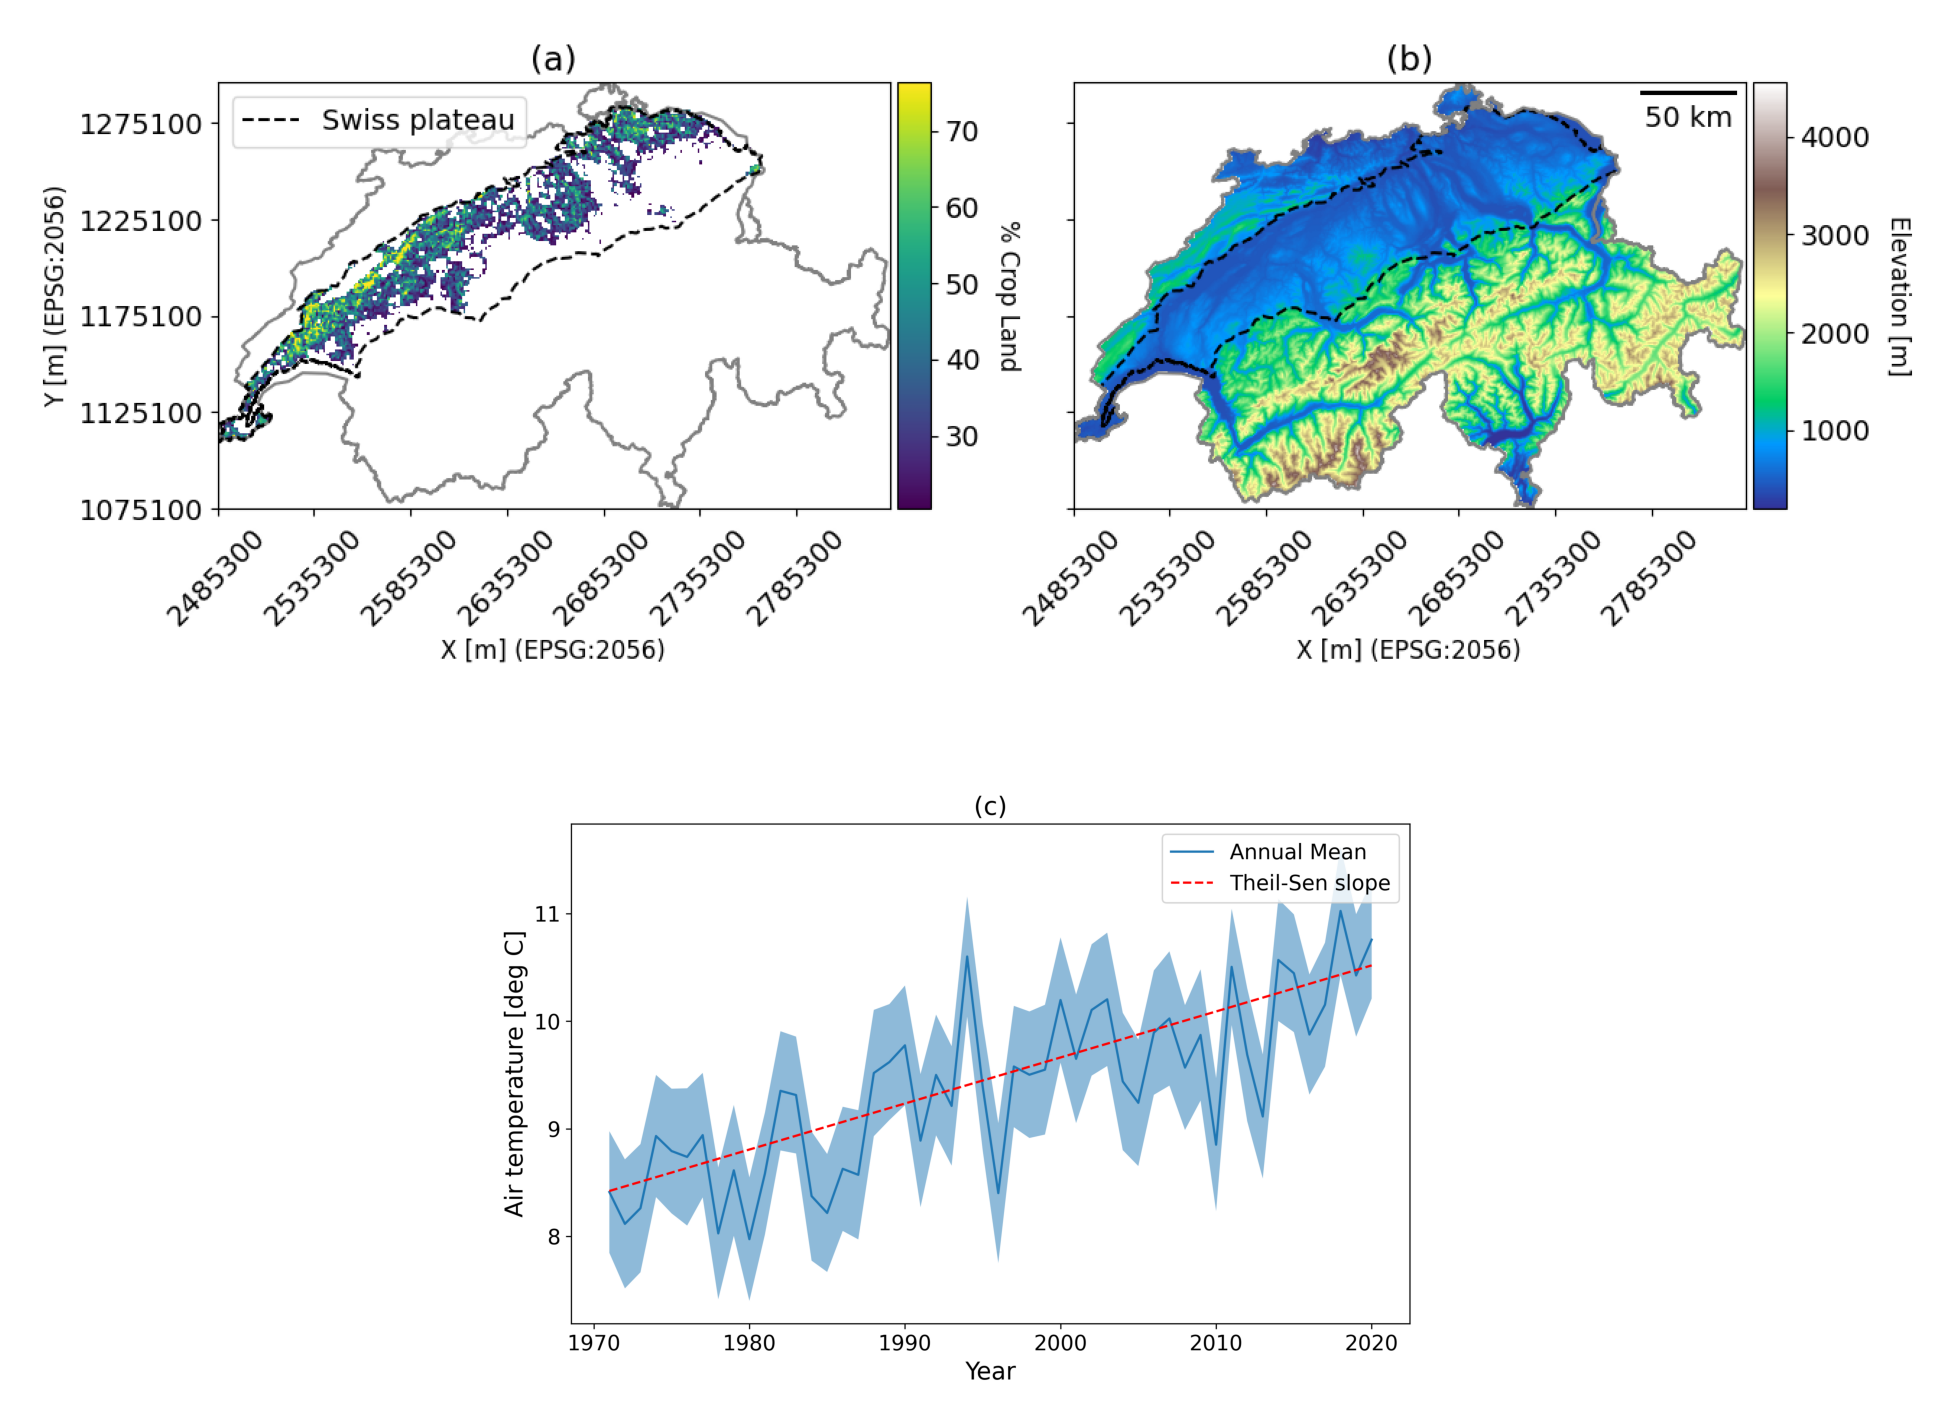
\includegraphics[width=\textwidth]{03-Heading-Dates/img/figure_study_area.png}
    \caption{Map of Switzerland with the spatial extent of the simulation defined by grid cells with more than 20\% of crop land (a) and elevation a.m.s.l. provided by the Swiss federal office of topography, SwissTopo (b). The annual average air temperature of the selected grid cells provided by the federal office of meteorology, MeteoSwiss, is shown in (c) including the standard deviation (filled blue area) and the Theil-Sen trend indicator (dashed line).}
    \label{fig:map-spatial-units}
\end{figure}

\subsection{Field phenotyping data}
\subsubsection{Selection of winter wheat varieties}
\label{subsubsec:varieties}
Two winter wheat varieties with different heading dates were selected: Arina and CH-Claro. According to long-term field trials conducted by the Swiss Federal Research Station Agroscope, Arina is a late variety in terms of ear emergence. Arina has been on the list of recommended varieties in Switzerland since 1981. CH-Claro, which has been on the recommended list since 2009, is a medium-early variety \citep{strebel_liste_2023}, i.e. ear emergence is slightly delayed compared to Arina. These two varieties therefore appear to be suitable for covering the expected range of heading dates in Switzerland and thus for landscape-scale simulation.

\subsubsection{Calibration data}
\label{subsubsec:hd-cal-data}
A multi-year and multi-site dataset collected as part of variety trials in the Swiss plateau between 2000 and 2018 was used for model calibration. The dataset has already been used in a previous study on the impact of projected climate change on winter wheat phenology by \cite{rogger_can_2021}. For Arina, a total of 104 heading date ratings were available from 14 locations and 19 years, covering the period between 2000 and 2018 (Table \ref{tab:cal-data}). 55 of these ratings are averages of two or more ratings with the same site and year. Heading date ratings for CH-Claro (N = 80, 47 as averages of two or more ratings) cover the years 2008 to 2018 at 10 locations (Table \ref{tab:cal-data}). The headline data were geocoded as \gls{DOY} at postcode level, as the exact location of the test sites was not disclosed. The central coordinate of the postcode zone was then used to extract the corresponding meteorological data from the gridded data product (section \ref{subsec:meteo}). Crops were cultivated extensively according to Swiss best practice for growth regulator and fungicide-free agriculture ("Extenso"). Fertilisation followed Swiss standards (GRUD, \cite{carlen_grundlagen_2017}). Further details on the data set can be found in \cite{rogger_can_2021}.

\begin{table}[H]
\caption{Calibration data used showing the number of location and years and the number of environments (site-year combinations).}
\centering
\label{tab:cal-data}
\begin{tabular}{@{}lllll@{}}
\toprule
\textbf{Variety}  & \textbf{Locations} & \textbf{Years} & \textbf{Year Range} & \textbf{Environments}   \\ \midrule
Arina    & 14        & 19    & 2000-2018  & 104 \\
CH-Claro & 10        & 11    & 2008-2018  & 80  \\ \bottomrule
\end{tabular}
\end{table}

\subsubsection{Validation data}
\label{subsubsec:hd-val-data}
For model validation, two independent datasets were available (Table \ref{tab:val-data}): A dataset containing historical heading date observations published by MeteoSwiss and a more recent dataset acquired during field phenotyping efforts.

\begin{table}[H]
\caption{Validation data used showing the number of location and years and the number of environments (site-year combinations).}
\centering
\label{tab:val-data}
\begin{tabular}{@{}lllll@{}}
\toprule
\textbf{Data Source}  & \textbf{Locations} & \textbf{Years} & \textbf{Year Range} & \textbf{Environments}   \\ \midrule
Field phenotyping    & 2        & 7    & 2016-2022 & 9 \\
Historical (MeteoSwiss) & 39        & 24    & 1972-1995  & 476  \\ \bottomrule
\end{tabular}
\end{table}

\paragraph{Field phenotyping data}
Multi-year heading date ratings of Arina and CH-Claro obtained at the FIP field phenotyping site \citep{kirchgessner_eth_2017} (47.449 N, 8.682 E; 556 m a.s.l., managed according to Swiss good agricultural practice ("ÖLN")) were used. For each of the two selected cultivars, 20 heading date ratings were available for seven consecutive years (2016-2022). In addition, in 2019, data from the variety trials conducted by Delley seeds and plants Ltd at Delley (46.918 N, 6.979 E; 500 m a.s.l., managed according to "Extenso" rules) could be used \citep{roth_image-based_2023}, providing four additional ratings per variety. Thus, a total of 9 environments (site-year combinations) were available. As for the calibration data, the meteorological data were extracted from the grid cell corresponding spatially to the site.

\paragraph{Historical ratings}
For the period 1972 to 1995, evaluations of the heading date of winter wheat were available from MeteoSwiss with a total of 476 environments (year-location combinations) scattered across Switzerland at altitudes ranging from 305 to 900 m. In detail, 39 different locations and 24 individual harvest years were included in the dataset. The exact location of the evaluated plots was not disclosed. Instead, the values for the nearest MeteoSwiss weather station were reported. Unfortunately, this dataset also lacked variety and management information, as well as quality indicators of the reliability of the observations.

\section{Methods}
\label{sec:hd-methods}
\subsection{In-situ rating of heading dates}
\label{subsec:rating-method}
In-situ heading date ratings were conducted by experts using visual scoring of the inflorescence. Heading was reached when half of the inflorescence emerged from the flag leaf sheath \citep{meier_growth_2018}. This rating scheme was used for both, calibration (Section \ref{subsubsec:hd-cal-data}) and validation data (Section \ref{subsubsec:hd-val-data}) except the MeteoSwiss dataset with historical ratings for which the methodology was not reported.

\subsection{Simulation of phenological development}
To simulate phenological development, the phenology module of the mechanistic crop model WOrld FOod STudies (WOFOST) -- hereafter referred to as the \gls{WOFOST} phenology model -- developed to simulate the growth and development cycle of cereal crops \citep{diepen_wofost_1989} was used. WOFOST-phenology has been shown to accurately predict the phenology of winter wheat in Europe \citep{ceglar_improving_2019} and therefore seems suitable for our study.
All simulations were performed using the Python Crop Simulation Environment\footnote{\url{https://github.com/ajwdewit/pcse}} (version 5.5.4) in Python 3.11.5.

The \gls{WOFOST} phenology model accumulates daily mean air temperature sums for each $i$th day after sowing between a base temperature $T_{base}$, below which no development is assumed, and a maximum effective temperature $T_{max, e}$, above which the development rate is set to a constant value. For winter wheat, $T_{base}$ is usually set to 0 deg C \citep{porter_temperatures_1999}. $T_{max,e}$ has been set to 30 degrees C as suggested by \cite{ceglar_improving_2019}. To reach anthesis, the \gls{WOFOST} phenology model constrains the accumulation of temperature sums by vernalisation and photoperiod.

\begin{equation}
\label{eq:dvs}
    DVS = \sum_i \frac{max(0, min((T_i-T_{base}), T_{max, e})}{T_{sum1}} \cdot V_{i} \cdot P_{i}
\end{equation}

In the equation \ref{eq:dvs}, $DVS$ represents the phenological development, $T_i$ the daily mean air temperature, $T_{sum1}$ the length of the vegetative growth period in effective degree days, $V_i$ the vernalisation and $P_i$ the photoperiod factor. $T_{sum1}$ is optimised for each winter wheat variety (see section \ref{subsec:hd-model-cal}). $V_i$ is based on daily mean air temperature using a dose-response approach proposed by \cite{wang_simulation_1998}. Cardinal temperatures for $V_i$ have been set to model defaults for winter wheat, as unfortunately adequate calibration data are not available for individual varieties. $P_i$ depends on day length, which is a function of latitude and Julian date, both given by the simulation inputs. $DVS$ is updated for each simulation step, i.e. each day after sowing, until anthesis is reached. Anthesis is reached when $DVS == 1$. As our calibration data contain heading dates instead of anthesis dates, which are the subsequent phenological development stage \citep{meier_growth_2018}, the simulation with the optimised $T_{sum1}$ parameter will output heading dates accordingly.

\subsection{Model Calibration}
\label{subsec:hd-model-cal}
We optimised the parameter $T_{sum1}$, which accounts for the length of the vegetative period (equation \ref{eq:dvs}), per winter wheat variety using the calibration data available from variety trials (see section \ref{subsubsec:hd-cal-data}, table \ref{tab:cal-data}). For optimisation, we minimised the \gls{RMSE} between all $n$ observed ($y$) and simulated ($\hat{y}$) heading data per variety in Python's \textsl{science.optimize.minimize} module (version 1.11.2) using the Constrained Optimisation by Linear Approximation (COBYLA) solver proposed by \cite{powell_efficient_1964}, which allows bound-constrained minimisation.

\begin{equation}
\label{eq:rmse}
    RMSE = \sqrt{\sum_{i=0}^n \frac{(\hat{y}_i - y_i)^2}{n}}
\end{equation}

Here, initial bounds for $T_{sum1}$ were set in the range of 700 to 900 effective \gls{GDD} based on empirical knowledge. The $T_{sum1}$ parameter value for which the RMSE between observed and modelled heading dates was smallest (equation \ref{eq:rmse}) was stored for each winter wheat variety. Table \ref{tab:tsum1-values} shows the obtained optimised $T_{sum1}$ parameter values per winter wheat variety, which were used in all subsequent model runs.

\begin{table}[H]
\caption{Optimized $T_{sum1}$ values per winter wheat variety.}
\label{tab:tsum1-values}
\centering
\begin{tabular}{@{}ll@{}}
\toprule
Variety  & $T_{sum1}$ [deg C] \\ \midrule
Arina    & 832   \\
CH-Claro & 795   \\ \bottomrule
\end{tabular}
\end{table}

\subsection{Model Validation}
The optimised \gls{WOFOST} phenology model was evaluated per winter wheat cultivar by comparing observed and simulated heading dates - expressed as \gls{DOY} - in terms of \gls{RMSE} (equation \ref{eq:rmse}), Pearson's $R$ and Spearman's rank correlation coefficient (Spearman's $rho$). We chose to use both correlation measures to quantify not only linear relationships between observed and simulated heading data (Pearson's $R$), but also monotonic relationships.

Validation was performed using the independent validation data (see section \ref{subsubsec:hd-val-data}), which were not used to optimise the $T_{sum1}$ parameter. For the field phenotyping data with known sowing dates and variety information, the \gls{WOFOST} phenology output could be used directly. In the case of the historical ratings provided by MeteoSwiss, we averaged the results of the two varieties and the two sowing date configurations (see next section, \ref{subsubsec:sowing-date-estimation}) into a single value, as the actual variety and sowing date were unknown.

\subsection{Model inference at the landscape scale}

\subsubsection{Sowing date estimation}
\label{subsubsec:sowing-date-estimation}
At the landscape scale, the exact sowing date is usually unknown. To overcome this problem, we used the sowing date estimation algorithm developed by \cite{holzkamper_spatial_2015}, which is based on empirical knowledge: Specifically, a temperature and precipitation criterion is used to identify suitable sowing dates within a predefined period when winter wheat is typically sown. This period was restricted to the time between October $7^{th}$ and November $7^{th}$ based on empirical knowledge of Swiss agricultural practice. During this period, a date is suitable for sowing if the mean air temperature was below 12 degrees C for 6 consecutive days and the sum of daily precipitation was less than 20, 16, 12, 8, 4 mm for 5 consecutive days. The first date meeting these criteria is used as the sowing date. While \cite{holzkamper_spatial_2015} reported a \gls{RMSE} of the sowing date estimation of 6 days considering a large number of observations (N = 258), internal tests with a smaller number of sites (N = 46) showed a larger \gls{RMSE} of 16 days. Furthermore, using only the first potentially suitable sowing date does not always seem appropriate, as the sowing date depends not only on the weather, but also on the availability of machinery, labour and inputs such as seed.

We therefore decided to use the first and last suitable potential sowing dates identified by the algorithm for our simulations. We assume that this captures all the temporal variability of sowing dates within a spatial unit.

\subsubsection{Model setup}
We used the 1 by 1 km grid cells (N = 5230, see section \ref{subsec:meteo}) constrained by the cropped area (see figure \ref{fig:map-spatial-units}a) to run the \gls{WOFOST} phenology simulations for the crop years 1972 to 2020. For each of the 5230 spatial units, simulations were run separately per winter wheat variety (N = 2), sowing date type (N = 2) and growing season (N = 49), resulting in a total of 1'025'080 \gls{WOFOST} phenology runs.

\subsubsection{Landscape-scale analysis}

To test for temporal trends in each spatial unit, we used the Theil-Sen trend estimator \citep{theil_rank-invariant_1950, sen_estimates_1968}, which is a non-parametric estimator of a linear trend. In detail, for a time series of $n$ simulated heading data $x_i$ ($1 = 1, \dots, n$), the Theil-Sen trend estimator computes the median of the slopes of all $i$, $k$ data pairs, $\beta$:

\begin{equation}
\label{eq:theil-sen}
    \beta = \underset{i < k}{median} \left(\frac{x_k - x_i}{k - i}\right)
\end{equation}
To infer the statistical significance of the obtained slope value $\beta$ (equation \ref{eq:theil-sen}), we used the Mann-Kendall test for monotonic trend \citep{mann_nonparametric_1945, kendall_rank_1975} as suggested by \cite{hu_earlier_2005}. Both trend estimation and testing were implemented using the open source Python library \textsl{pyMannKendall}. \citep{hussain_pymannkendall_2019}, available under the MIT licence. To avoid finding significant results by chance due to a large number of spatial units, we adjusted the obtained significance values using the Benjamin-Hochberg correction \citep{benjamini_controlling_1995} with a false discovery rate of 0.05 implemented in the open source Python \textsl{statsmodels} library \citep{seabold_statsmodels_2010} (version 0.15.0) available under modified BSD (3-clause) licence.


\section{Results}
\label{sec:hd-results}
\subsection{Validation}
\subsubsection{Field phenotyping data}
\label{subsubsec:res-phenotyping}
Figure \ref{fig:val-scatter} shows the scatter plots of observed versus simulated heading dates expressed as \gls{DOY} for Arina (Figure \ref{fig:val-scatter}a) and CH-Claro (Figure \ref{fig:val-scatter}b), colour-coded by harvest year. In both cases the simulation was in good agreement with the desired one-to-one light (dashed line), resulting in a \gls{RMSE} of 2.11 and 1.79 for Arina and CH-Claro respectively. Pearson's $R$ was high for both varieties (0.97 and 0.91 respectively), with a higher Spearman's $rho$ for Arina (0.98) than for CH-Claro (0.70). This means that the model was able to accurately predict the heading date and resolve differences in the timing of heading between the years.

CH-Claro reached the heading stage slightly earlier than Arina in both the observed and simulated heading dates: The observed mean difference between Arina and CH-Claro was about 2.1 days compared to 1.8 days in the simulation results.

\begin{figure}[H]
    \centering
    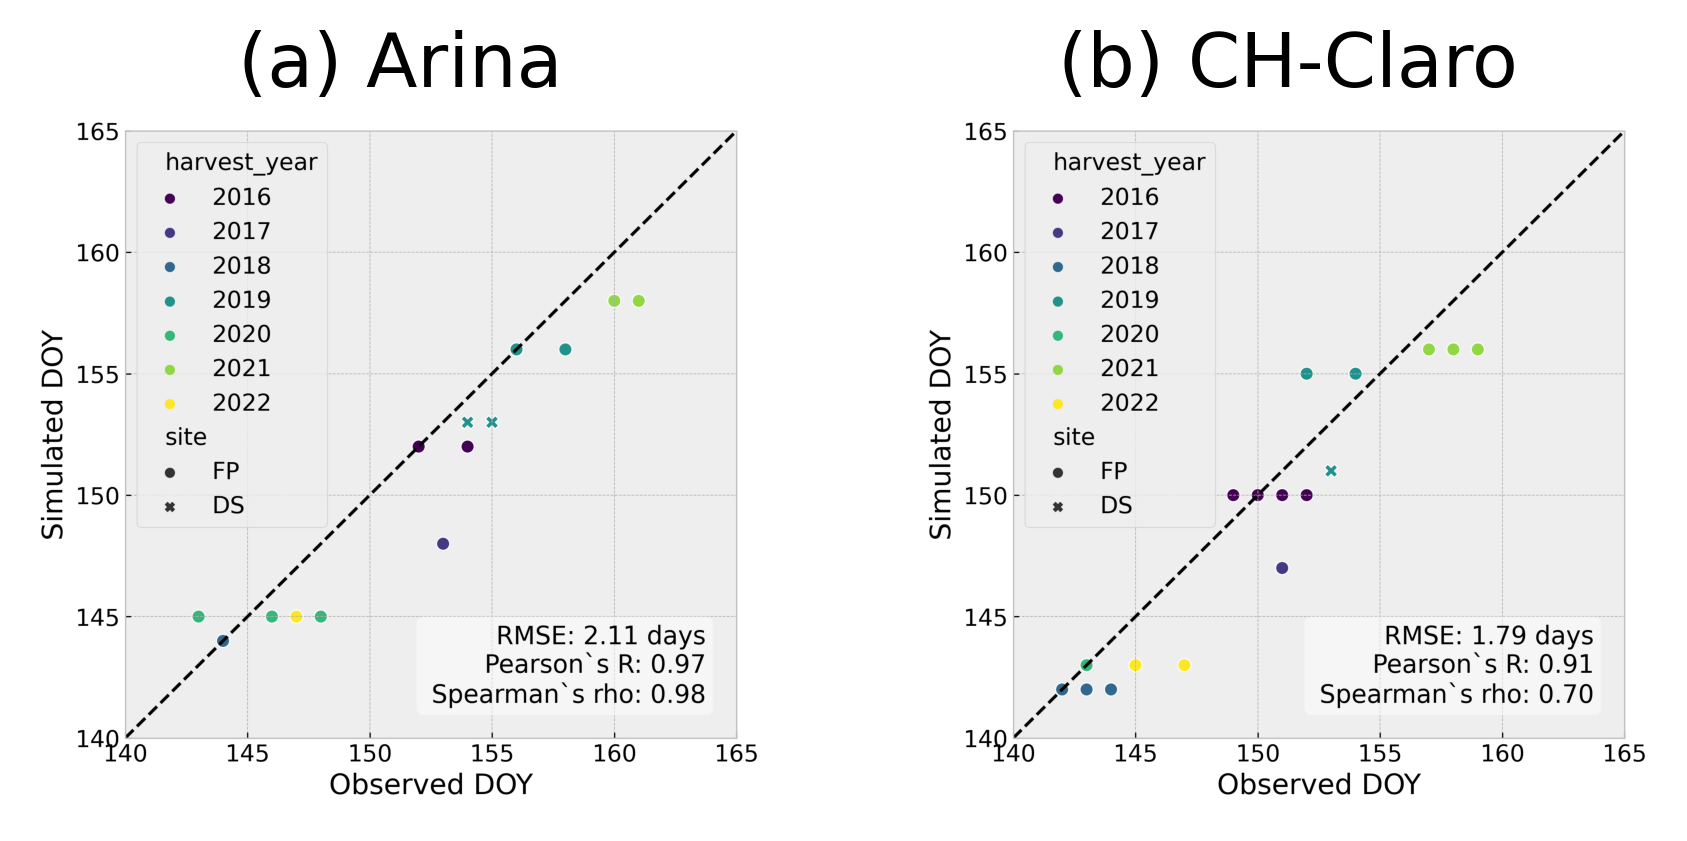
\includegraphics[scale=0.7]{03-Heading-Dates/img/scatter_plot_validation_phenotyping.png}
    \caption{Scatter plot of observed and simulated heading dates for Arina (a) and CH-Claro using the independent validation data set at the FIP and Delley site color-coded by harvest year (N = 24).}
    \label{fig:val-scatter}
\end{figure}

\subsubsection{MeteoSwiss historical dataset}
\label{subsubsec:meteoswiss-data}

The scatter plot with the validation results from the MeteoSwiss historical dataset is shown in Figure \ref{fig:val-scatter-meteoswiss}. The offset from the desired 1:1 line (dashed line in Figure \ref{fig:val-scatter-meteoswiss}) was greater than for the field phenotyping data (section \ref{subsubsec:res-phenotyping}), resulting in a \gls{RMSE} of 10.9 days. Both Pearson's $R$ and Spearman's $rho$ were around 0.5 at the 0.001 significance level.

\begin{figure}[H]
    \centering
    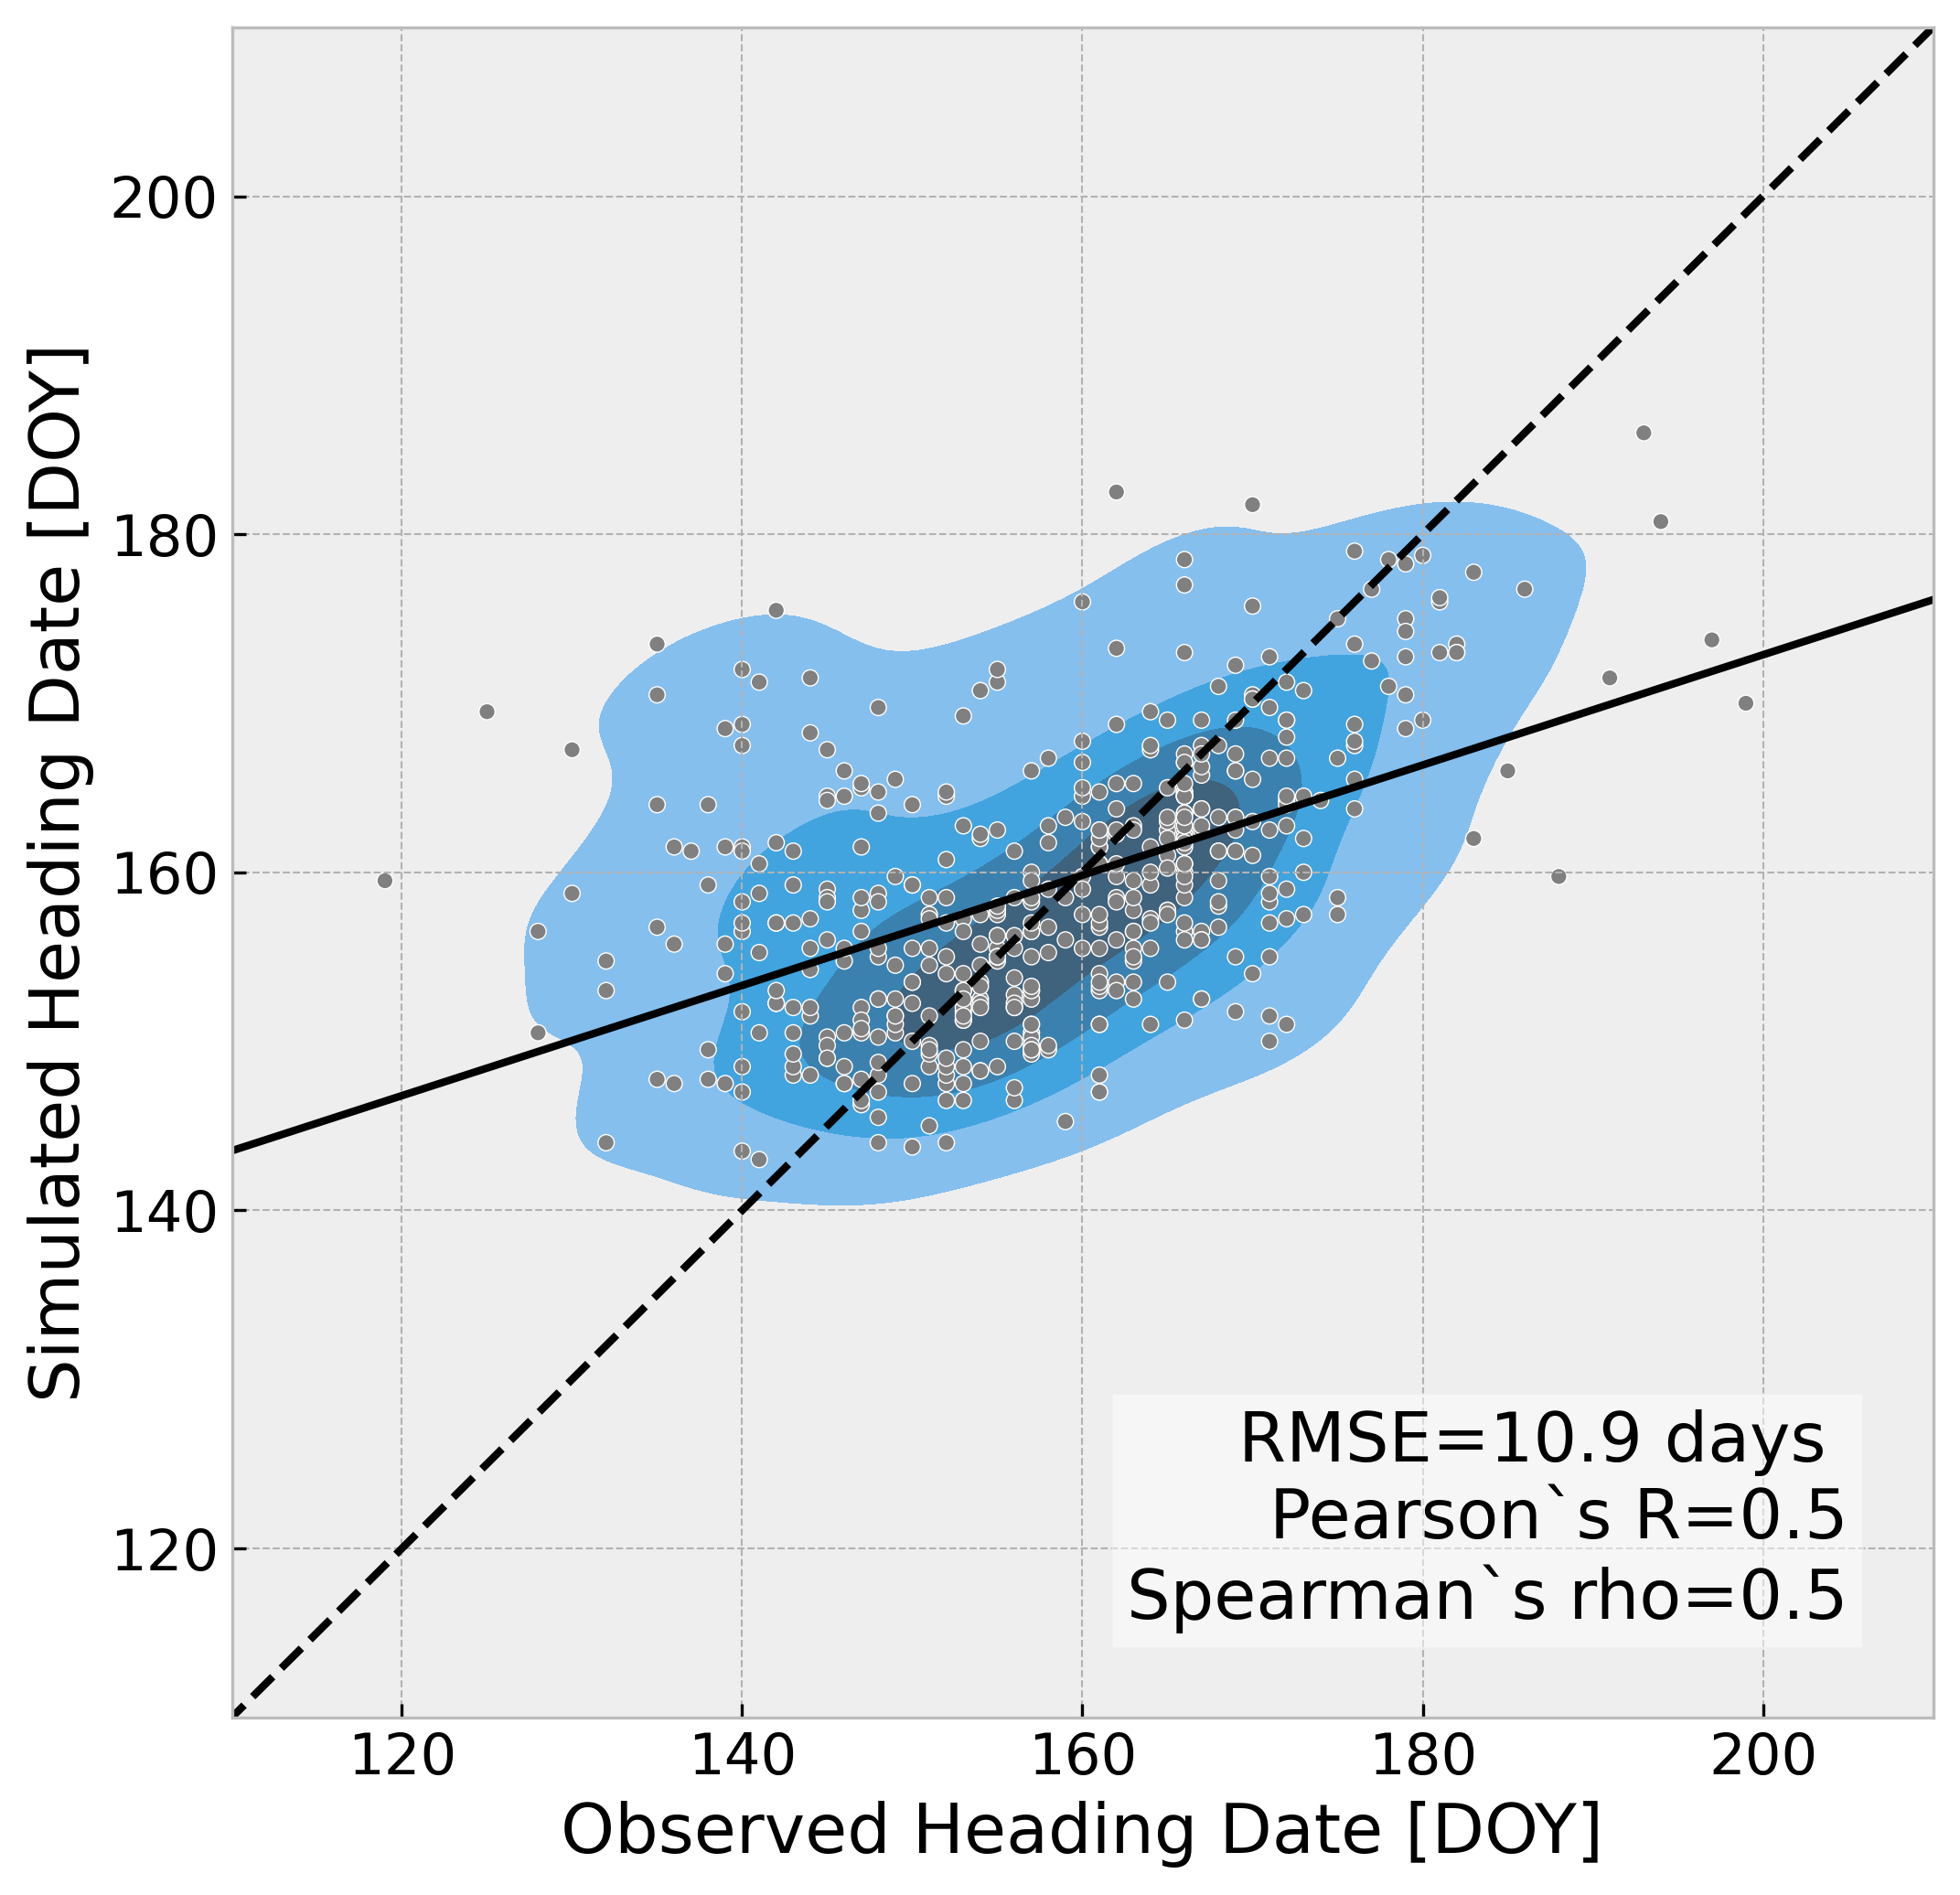
\includegraphics[scale=0.5]{03-Heading-Dates/img/scatter_plot_validation_meteoswiss.png}
    \caption{Scatter plot of observed and simulated heading dates using the MeteoSwiss historical validation data set for the years 1972 to 1995 (N = 415).}
    \label{fig:val-scatter-meteoswiss}
\end{figure}

\subsection{Landscape-scale analysis}

\subsubsection{Sensitivity to the sowing date}
\label{subsubsec:sensitivity}

For sensitivity analysis, the differences between the latest and earliest sowing dates by genotype are shown in Figure \ref{fig:sowing-date-sensitivity}. The box plots of the differences per crop year (Figure \ref{fig:sowing-date-sensitivity}a, c) show that the differences were systematically $\ge$ 0 days for all years. There was no pronounced difference between Arina and CH-Claro and only small variability between years. Most differences were between 0 and 3 days, as shown by the frequency distributions (see histograms in Figure \ref{fig:sowing-date-sensitivity}b, d). Only a few data points ($\le$ 1\% of the values) showed differences between the two sowing dates of 4 days or more. Therefore, in the forthcoming results we show simulations run with the earliest sowing date only.

\begin{figure}[H]
    \centering
    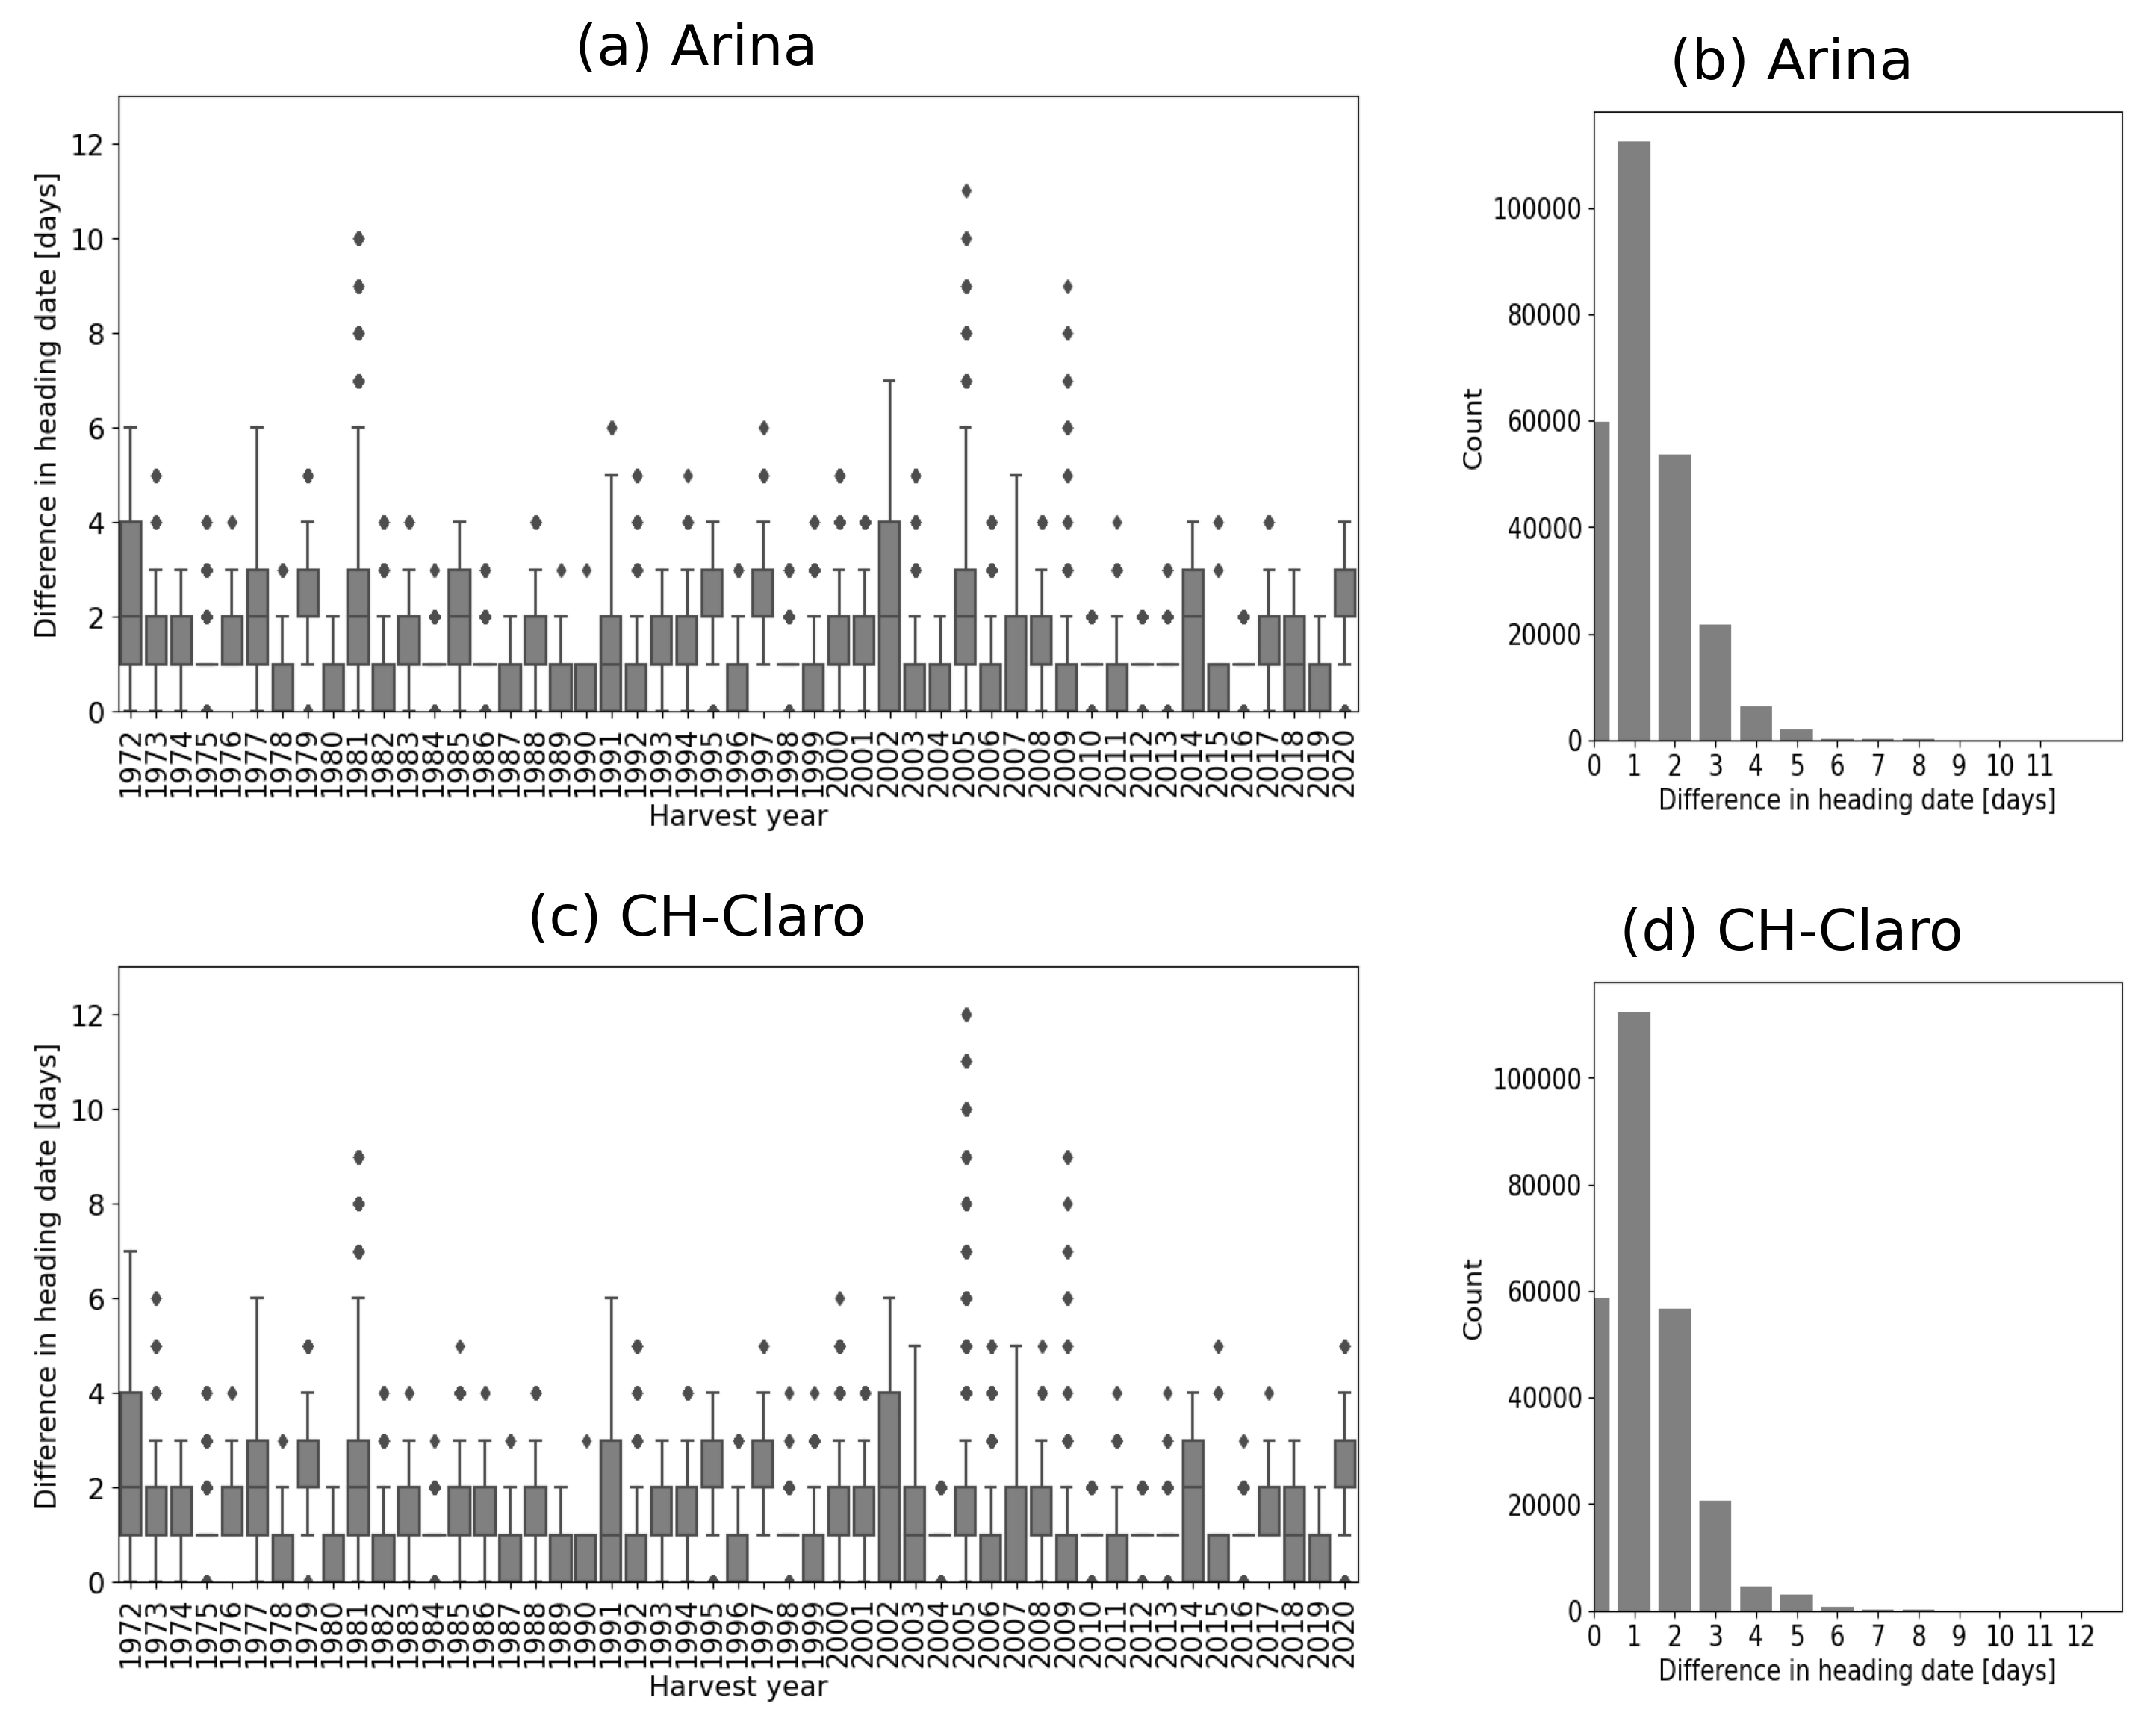
\includegraphics[width=\textwidth]{03-Heading-Dates/img/sowing_date_sensitivity.png}
    \caption{Box plots per harvest year (a, c) and histograms (b, d) of the differences in heading date between the latest and earliest sowing date for Arina and CH-Claro.}
    \label{fig:sowing-date-sensitivity}
\end{figure}


\subsubsection{Spatial analysis}

Figure \ref{fig:median-heading-map}a-b shows the median of simulated heading dates per grid cell between 1971 and 2020 and the corresponding frequency distribution. Median heading dates for Arina in the study area ranged between \gls{DOY} 146 and 171 (mean \gls{DOY}: 155.5, median \gls{DOY}: 155, standard deviation: 3.8 days). The median \gls{DOY} for CH-Claro was between 144 and 169 (mean \gls{DOY}: 153, median \gls{DOY}: 153, standard deviation: 3.6 days). The central 50\% of the median heading date values were between \gls{DOY} 153 and 158 for Arina, and \gls{DOY} 150 and 155 for CH-Claro (see histograms in Figure \ref{fig:median-heading-map}). Lower \gls{DOY} were simulated for both varieties in southwestern and northeastern Switzerland (Figure \ref{fig:median-heading-map}a, b), with consistent spatial patterns. Overall, the two cultivars differed in the timing of the median heading date by 1 to 4 days.

The spread between the 25\% and 75\% quantile per grid cell for the years 1971 to 2020 (Figure \ref{fig:median-heading-map}c-d) showed values varying within the study area between 7 and 13 days for Arina (mean: 9.5, median: 9, standard deviation: 0.7 days) and between 7 and 12 days (mean: 9.5, median: 9, standard deviation: 0.7 days) for CH-Claro. There was a slight dependence of the interquantile range on the median elevation value per grid cell (Figure \ref{fig:median-heading-map}e): Grid cells with higher elevations tended to have slightly larger inter-quantile ranges. However, the linear relationship seems to be weak (Pearson's $R$ about 0.51). This result was the same for both varieties and is therefore only shown for Arina.

Figure \ref{fig:median-heading-map}f shows the scatterplot of median heading dates versus elevation values for Arina. There was a strong positive linear correlation (Pearson's R 0.83, significance level 0.001) between median elevation and median heading date: the higher the elevation, the later the heading date. Specifically, for the most frequent range of median elevation values (400 to 600 m), the median heading date for Arina was between \gls{DOY} 146 and 161 (Figure \ref{fig:median-heading-map}f). For CH-Claro, the linear relationship gave the same correlation coefficient and therefore the significance level is not repeated here.

\begin{figure}[H]
    \centering
    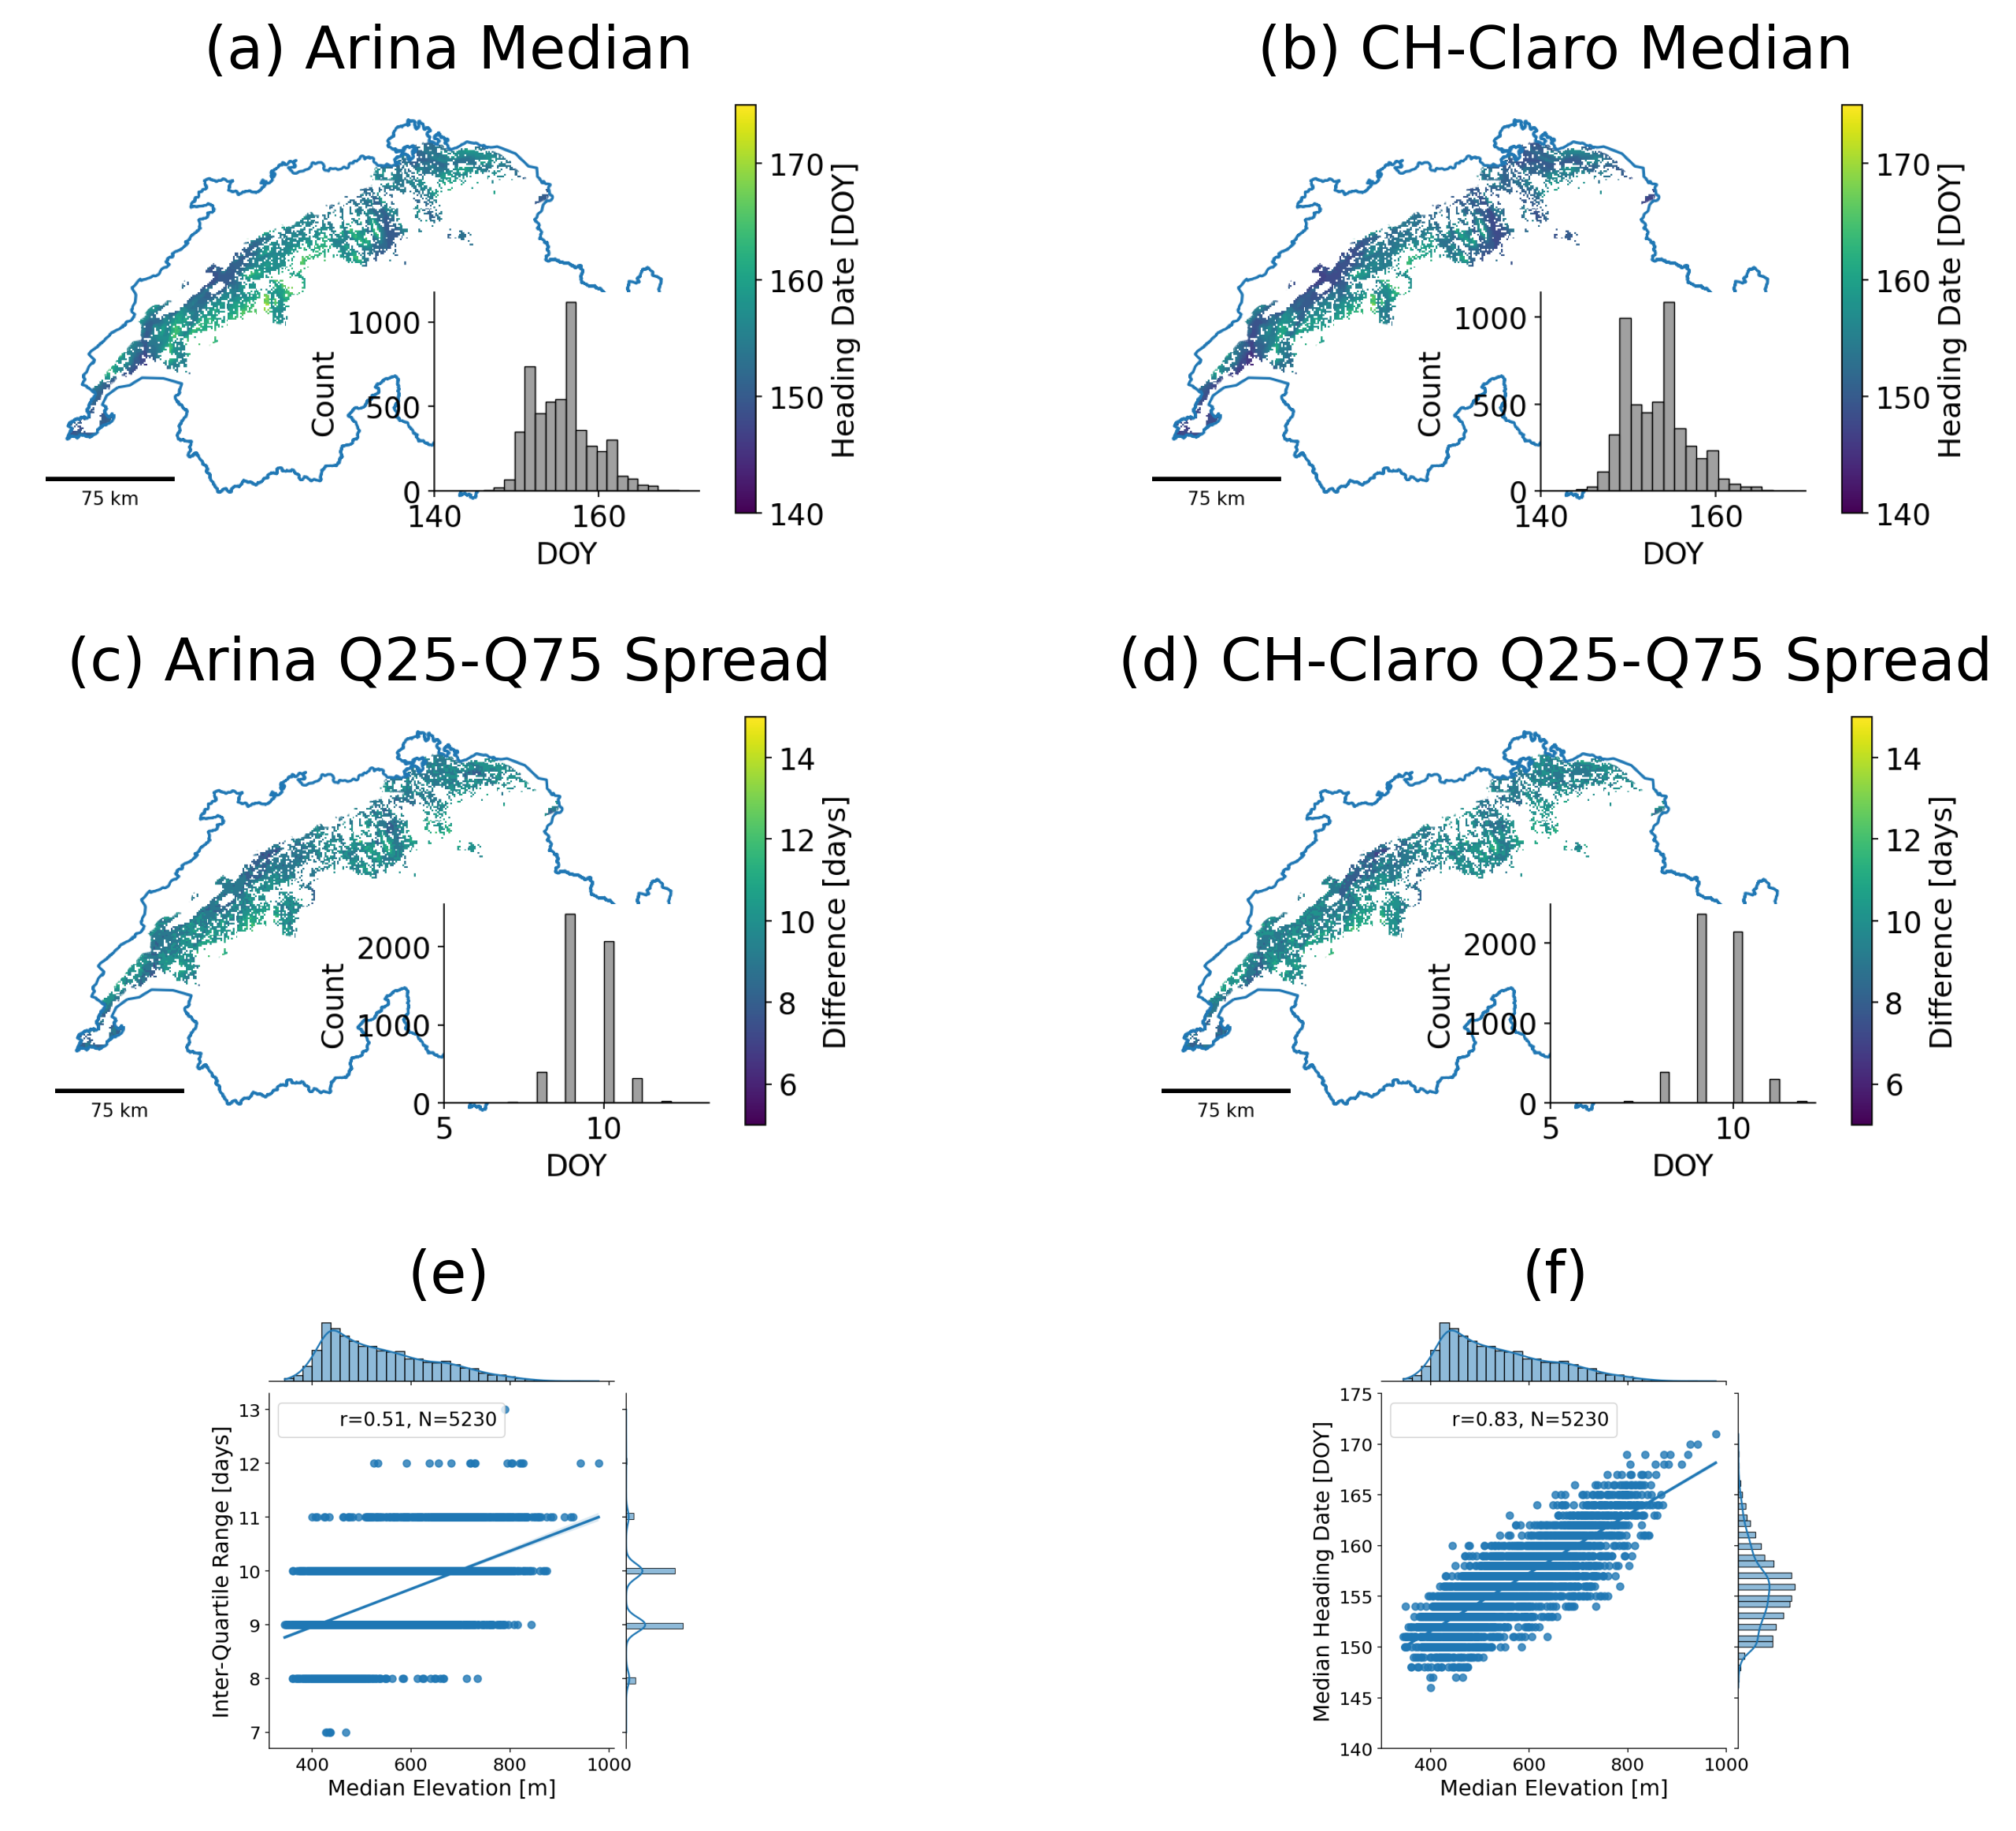
\includegraphics[width=\textwidth]{03-Heading-Dates/img/stats_map.png}
    \caption{Maps and histograms of the median heading date for the period 1971 to 2020 expressed as \gls{DOY} for Arina (a) and CH-Claro (b), and the interquantile range between the 25\% (Q25) and 75\% (Q75) quantiles (c-d; N = 5230). In addition, the scatterplot of the median heading date against the median elevation (e) and the interquantile range against the median elevation (f) is shown for Arina. The dependence on elevation was very similar for CH-Claro and is therefore not shown.}
    \label{fig:median-heading-map}
\end{figure}


\subsubsection{Temporal analysis}
\label{subsubsec:temp-analysis}
Figure \ref{fig:heading-boxplots-ts} shows box plots of simulated heading dates expressed as \gls{DOY} for Arina and CH-Claro (Figure \ref{fig:heading-boxplots-ts}a) and the differences between the varieties (Figure \ref{fig:heading-boxplots-ts}b) by harvest year considering all grid cells (N = 5230). There was a clear year-to-year variability in heading dates. Differences ranged from early (e.g. in 2007, 2011 or 2020) to late heading dates (e.g. in 1984 or 1987), with differences in median heading dates of up to 25 days when considering, for example, the difference between 2007 and 1984. The annual spread of heading date values, i.e. the spatial variability per harvest year, also differed slightly between years.

When comparing the two varieties, Arina systematically showed later heading dates than CH-Claro (Figure \ref{fig:heading-boxplots-ts}a). The differences between Arina and CH-Claro were between 1 and 4 days in most years (Figure \ref{fig:heading-boxplots-ts}b), with the majority of differences between 2 and 3 days. In 18 out of 49 years, the difference reached up to 5 days in a few outliers. In only 3 years the smallest difference was 2 days, compared to 1 day in the remaining years.

\begin{figure}[H]
    \centering
    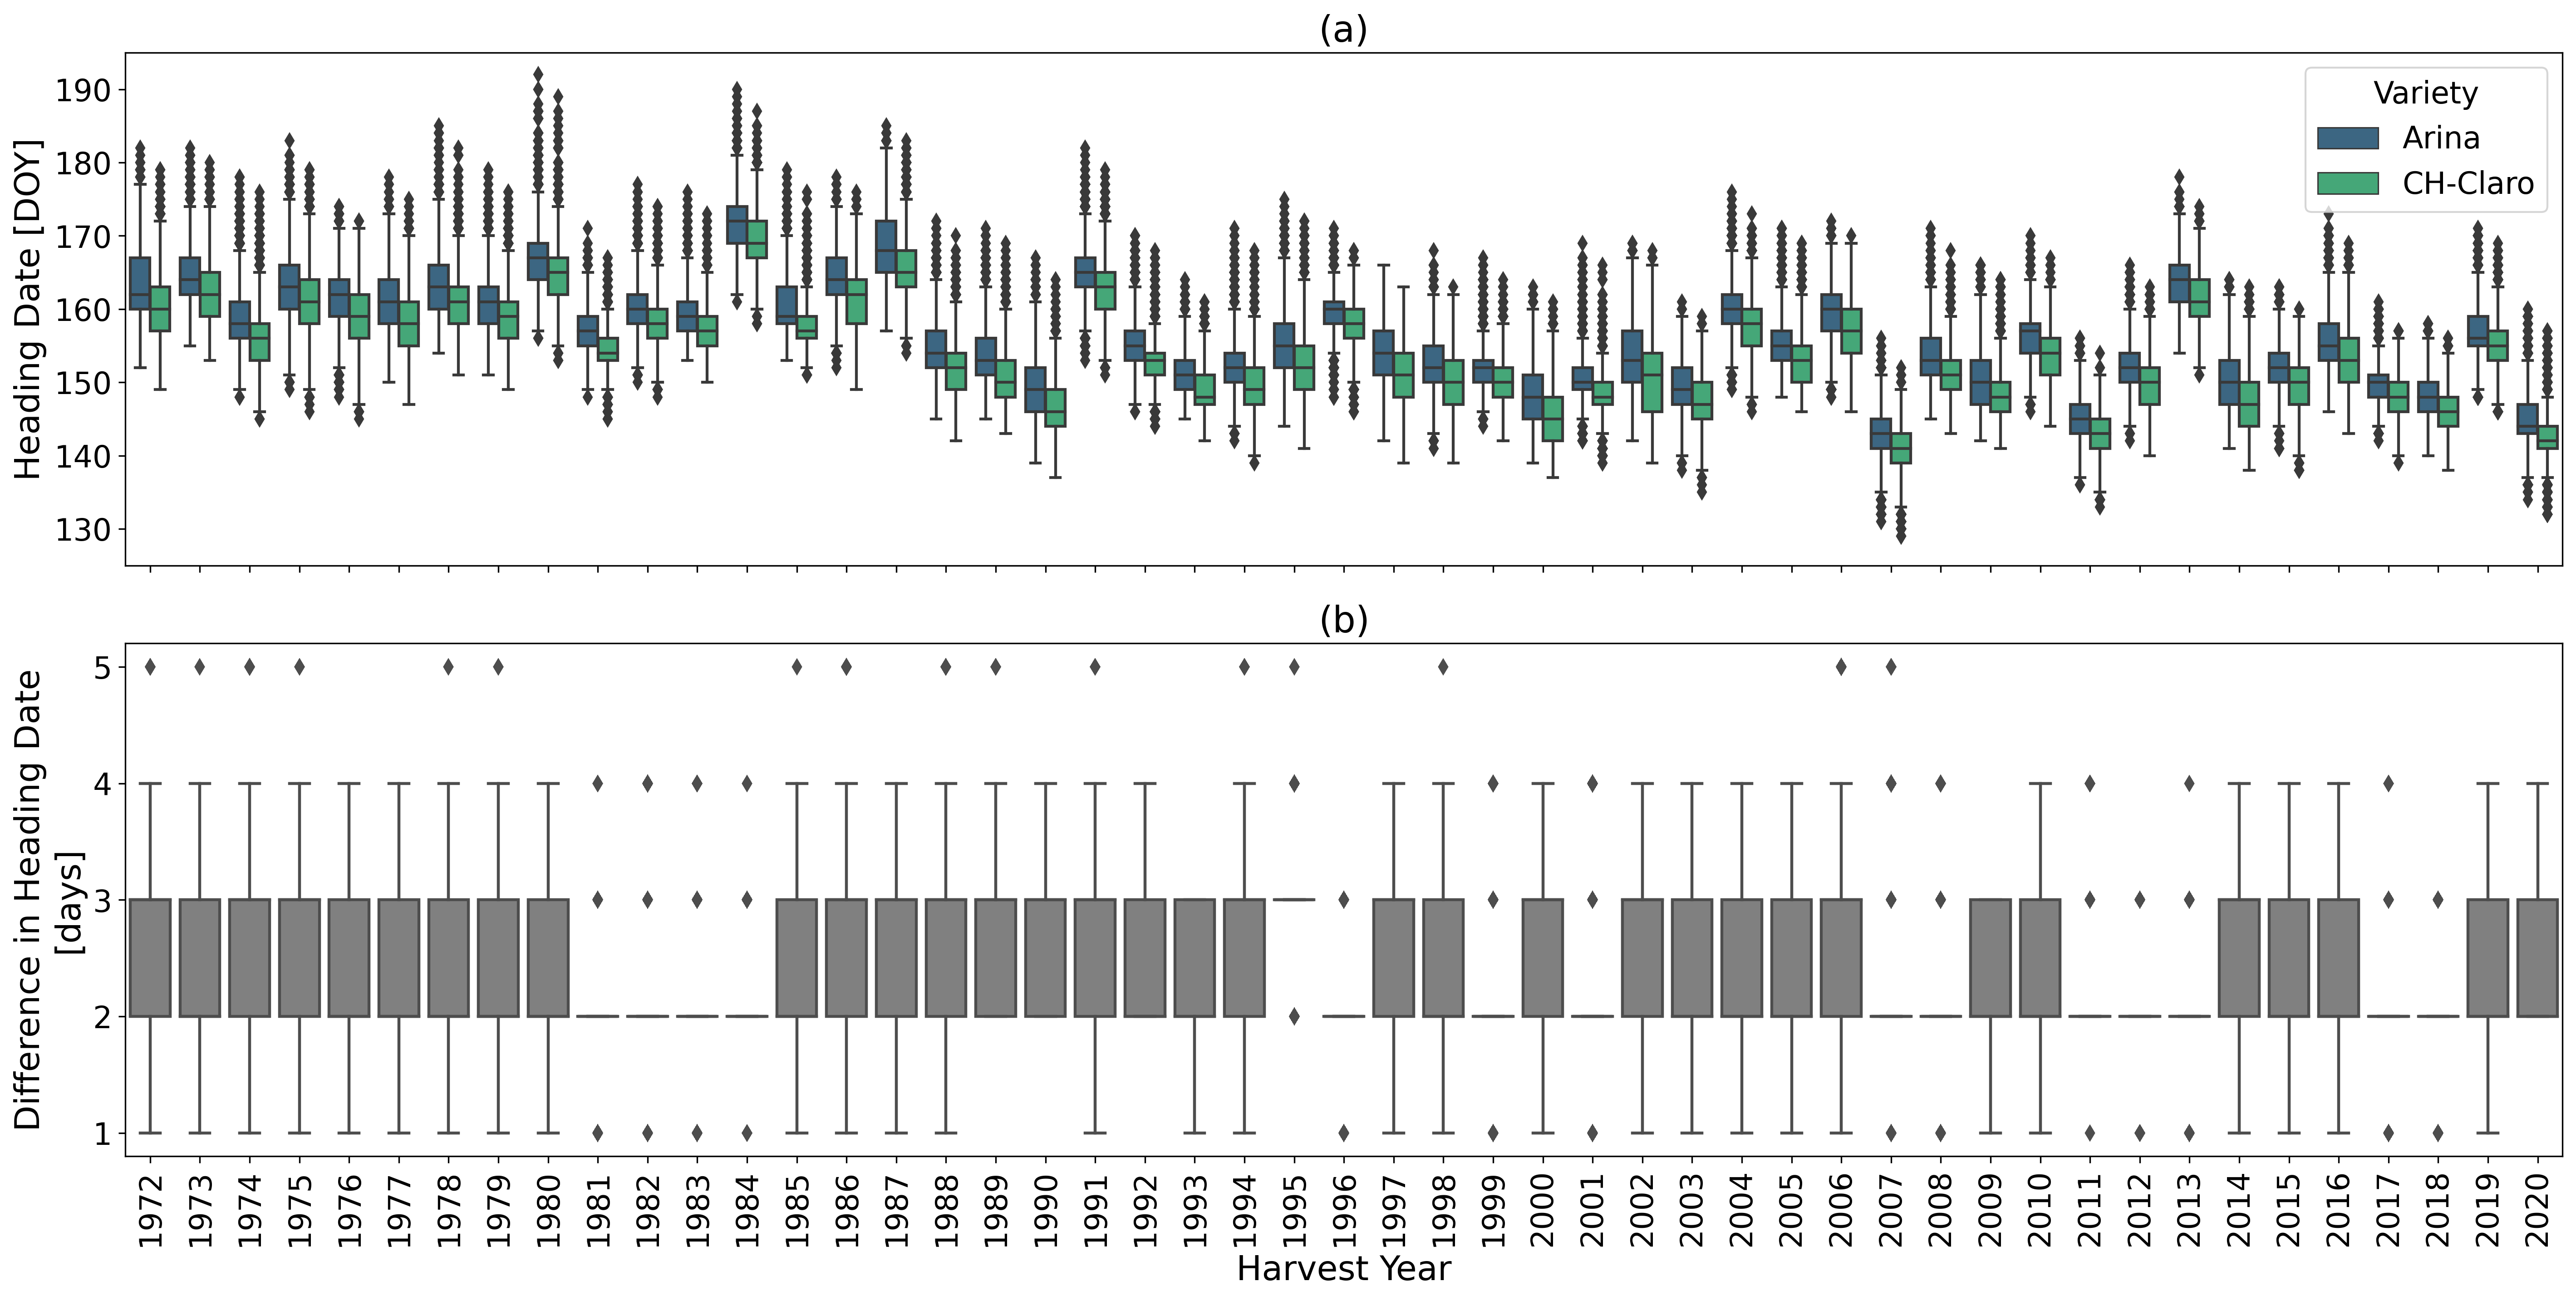
\includegraphics[width=\textwidth]{03-Heading-Dates/img/heading_boxplot.png}
    \caption{Box plots of simulated heading dates for Arina and CH-Claro by harvest year (a) and box plots of the differences in the timing of the heading date between Arina and CH Claro by harvest year(b) considering all grid cells (N = 5230).}
    \label{fig:heading-boxplots-ts}
\end{figure}

Based on the trend analysis, maps of the slope values obtained from the Theil-Sen trend estimator are shown in Figure \ref{fig:map-temporal-trend}a-b by variety. The trend values ranged from -0.43 to -0.16 $DOY/year$ for Arina (mean: -0.29 $DOY/year$, median: -0.3 $DOY/year$, standard deviation: 0.03 $DOY/year$). CH-Claro showed the same range of trend values (mean: -0.29 $DOY/year$, median: -0.29 $DOY/year$, standard deviation: 0.03 $DOY/year$). This means that in 2020 the heading occurred up to 14 days earlier than in 1971, assuming a trend value of -0.28 $DOY/year$. The spatial pattern of the trend values mirrored the pattern of the median heading date (Figure \ref{fig:median-heading-map}a, b). All trend estimates were significant at the 0.01 level according to the Mann-Kendall tests performed per grid cell.

\begin{figure}[H]
    \centering
    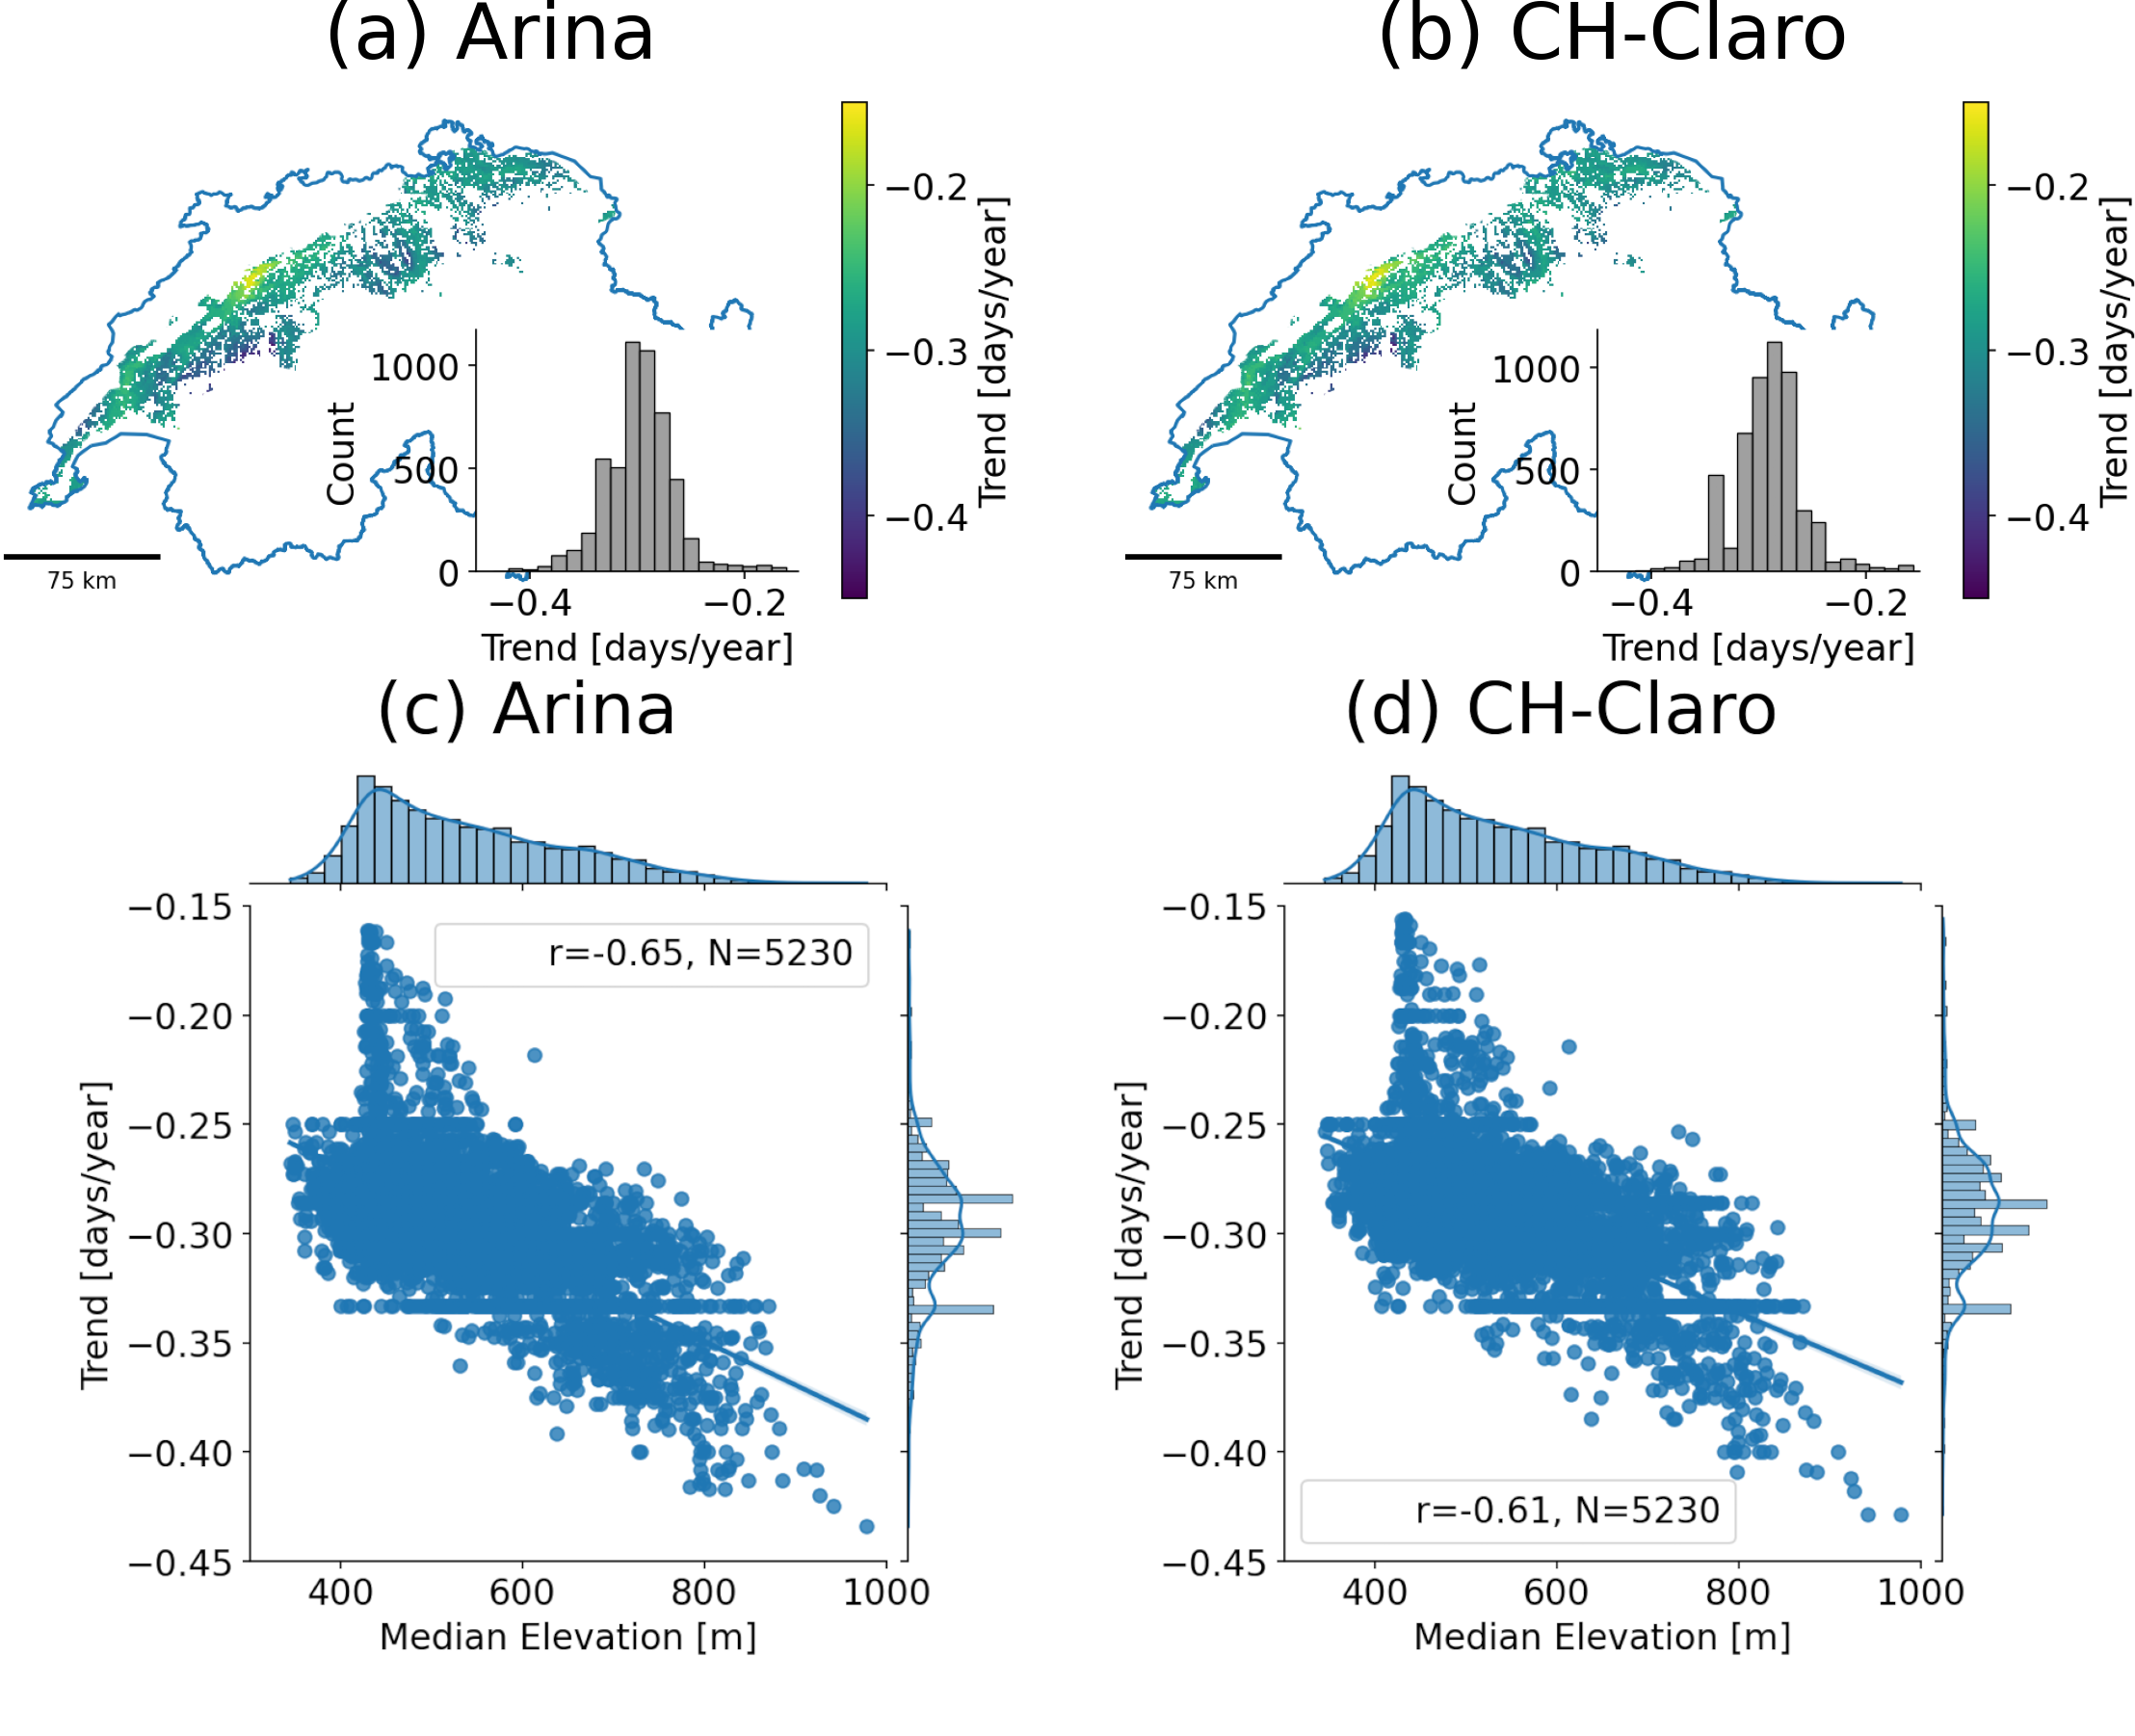
\includegraphics[width=\textwidth]{03-Heading-Dates/img/climate_signal_combined.png}
    \caption{Maps and histograms of the detected temporal trend in heading dates per grid cell (N = 5230) for Arina (a) and CH (b), and scatter plots of median elevation and trend values (c, d).}
    \label{fig:map-temporal-trend}
\end{figure}

Figure \ref{fig:map-temporal-trend}c-d shows the correlation between trend and median elevation similar to figure \ref{fig:median-heading-map}e-f. The correlation with the median elevation per grid cell was negative, i.e. the trend was more negative at higher elevations than at lower elevations (Pearson's R about -0.65 and -0.61 for Arina and CH-Claro, respectively, significance level: 0.01). The trend values $\le$ -0.4 were mainly observed at the mean altitude $\ge$ 800 m. At lower altitudes ($\le$ 500 m) the spread of the trend values is largest, ranging from -0.34 to -0.15 for both varieties.


\section{Discussion}
\label{sec:hd-discussion}
\subsection{Interpretation of results}
\subsubsection{Model performance}
The \gls{WOFOST} phenology model allowed an unbiased variety-specific prediction of heading date over several years at the phenotyping sites, as indicated by high values of Spearman's $rho$ and Pearson's $R$ (section \ref{subsubsec:res-phenotyping}). The model showed consistent differences in the timing of heading between Arina and CH-Claro, reflecting the expected differences between these two varieties known from in-situ observations. In addition, the inter-annual variability was reflected with good agreement with in-situ observations, as indicated by high values of the rank correlation coefficient (Figure \ref{fig:val-scatter}). The obtained \gls{RMSE} (2 days) was in good agreement with values reported in the literature: \cite{liu_uncertainty_2018}, for example, reported a \gls{RMSE} of 3 to 4 days for variety-specific prediction of wheat heading dates in China. \cite{rogger_can_2021}, who used the same data set for calibration as in this study (section \ref{subsubsec:hd-cal-data}) but focused on different varieties, reported \gls{RMSE} values of 3.6 days.

The results of the comparison with the historical MeteoSwiss data showed a reduced accuracy (see section \ref{subsubsec:meteoswiss-data}) with slightly higher errors of 11 days (see Figure \ref{fig:val-scatter-meteoswiss}). There are two main reasons for this: First, the data do not contain quality information. Thus, it is unclear whether all ratings were made according to the proposed methodology (see section \ref{subsec:rating-method}), which could be a potential source of discrepancy between observed and simulated heading dates. Secondly, as neither the sowing date nor the variety was known, the uncertainty arising from these unknowns limits the achievable error. As we have shown, both variety and sowing date have a small effect on the simulated heading date. Thus, part of the error in validating the historical ratings could be explained by the lack of management information mentioned above. It is also conceivable that small-scale microclimatic effects play a role. Indeed, we were able to show with the field phenotyping data that high accuracy is possible with the 1 on 1 $km^2$ grid cells. However, this is only a study using two grid cells (FIP and Delley) and is not necessarily representative of other locations. Overall, all three effects mentioned above are likely to contribute to the reduced accuracy of the validation of the Meteoswiss data.

Nevertheless, the model is arguably an appropriate tool for estimating variety-specific timing of heading dates in winter wheat and reflected inter-annual variability in heading dates with reasonable accuracy, as the magnitude of potential errors was clearly smaller than the spatio-temporal signal (research question one).

\subsubsection{Effect of the sowing date}
The effect of sowing date on simulated heading date was small (0 to 3 days) with little variation between years (see Figure \ref{fig:sowing-date-sensitivity}). Thus, knowledge of the exact sowing date seems to be less critical for predicting heading dates in winter wheat. We attribute this low sensitivity mainly to the non-linearity of the model due to the need for vernalisation and photoperiodism: Vernalisation in Switzerland mainly occurs in the winter months (December and January), which is well after the sowing period (October and November). This decouples the vernalisation event from the time of sowing. As vernalisation is required in winter wheat to enter the reproductive growth stage in the spring, the timing of the heading date is controlled more by the timing of the vernalisation event than by the time of sowing. Similarly, photoperiodism, i.e. the dependence of the phenological development of winter wheat on day length, is also likely to have a decoupling effect \cite{fedorov_photoperiodism_1976}.

Thus, the error due to uncertainty in the exact sowing date is much smaller than the year-to-year variability (Figure \ref{fig:heading-boxplots-ts}) and the range of simulated dates within the study area (Figure \ref{fig:median-heading-map}) (second research question). However, it is important to remember that earlier phenological stages - namely emergence - or other traits such as yield are known to be more dependent on the date of sowing \citep{ceglar_improving_2019, dueri_simulation_2022}, which then require a more accurate estimation of the timing of sowing events. Remote sensing based approaches using, for example, high resolution satellite constellations could provide the desired accuracy in predicting sowing dates \citep{sadeh_sowing_2019}.

\subsubsection{Spatio-temporal analysis}
The model allowed the spatially continuous simulation of heading dates. The observed spatial variability of median heading dates (Figure \ref{fig:median-heading-map}), but also the differences between years (Figure \ref{fig:heading-boxplots-ts}), clearly show that a spatially high-resolution simulation of phenology is important to quantify the totality of spatio-temporal variability in agricultural landscapes. In particular, landscapes with relatively small-scale changes in topography show clear gradients related to the general decrease in air temperature with altitude (Figure \ref{fig:median-heading-map}f). Differences in photoperiod are less significant due to the small spatial extent of the study region (Figure \ref{fig:map-spatial-units}). Consequently, weather conditions could cause pronounced differences between years, which should be taken into account, for example, when comparing plant growth between years.

The clear trend towards earlier heading dates is a clear consequence of the warming that has already occurred in Switzerland in recent decades (third research question, see Figure \ref{fig:map-spatial-units}c). Especially the higher altitudes have experienced the largest shifts (see Figure \ref{fig:map-temporal-trend}c-d). This is consistent with the finding that higher elevations in the Alps, but also in the Alpine foothills, are warming faster than lower elevations \citep{gusewell_changes_2017}. Our results show that the increase in air temperature of +2°C between 1971 and 2020 resulted in a systematic shift of about 14 days towards earlier departure dates. The results are consistent with an older study by \cite{hu_earlier_2005}, which observed changes between 0.8 and 1.8 days per decade in the Great Plains of the USA between 1935 and 2004, with similar spatial variation, and work by \cite{tariq_impact_2018} on sunflower phenology in Pakistan. In addition, our results confirm the findings of \cite{rogger_can_2021}, who predicted a shift towards earlier heading under climate change scenarios. This reiterates the importance of accurately estimating phenology to compare plant growth conditions across years and to develop a holistic understanding of plant growth and development in a warming climate.

\subsection{Limitations and ways forward}
The simulation focused on two winter wheat varieties used in Swiss agriculture. It does not fully take into account site-specific variety selection and breeding progress. In particular, the selection of varieties for cultivation at higher altitudes may require the use of different wheat varieties than in the lowlands. As we lack data on the geographical distribution of wheat varieties in Switzerland, we cannot make any conclusive statements in this respect. It is also conceivable that climatic factors or changes in agricultural practices may cause shifts in sowing dates, which we have not assumed in this study. It has been shown that due to continuous breeding progress, modern wheat varieties have an accelerated phenological cycle with reduced temperature sum requirements to reach flowering \citep{rezaei_climate_2018}. As Arina has been cultivated in Switzerland since the early 1980s, our findings are certainly relevant to Swiss agricultural practice. However, simulation studies over long periods should not ignore breeding progress, as phenology is also determined by genetic factors \citep{hyles_phenology_2020}. The same applies to agricultural management practice, although the lack of detailed management information currently limits the accuracy that can be achieved. Another point to consider is stressors \citep{perdomo_effects_2015}. The simulation of heading dates did not include heat or drought stressors, which could affect the phenological development of wheat.

In addition to these points, further research could investigate the spatio-temporal dynamics of other important phenological phases, such as the onset of stem elongation and senescence. However, the onset of stem elongation is time and labour intensive to monitor in situ. Therefore, comparatively little data is available to calibrate and validate models. The same is true for senescence. Overall, data availability is one of the major limiting factors for such studies. As most variety testing programs collect data on phenology, it would be welcome if more of these data were made openly available.

\section{Conclusion}
Variety-specific simulations of heading dates in two Swiss winter wheat varieties revealed past landscape-scale spatial variability and temporal trends. The observed high degree of spatio-temporal variability in heterogeneous landscapes highlights the contribution of phenology models to the assessment of climate change impacts and the comparison of crop growing conditions between years and sites. While the lack of accurate sowing date information had little effect on simulated heading dates due to vernalisation and photoperiodism requirements, recent changes in wheat variety selection and management practices may require further calibration and adaptation of the approach. Nevertheless, the approach presented provides a tool for assessing the impacts of climate change on crop production, which is relevant to agricultural practitioners and decision makers.

\section*{Code and Data Availability}
Code to re-run the \gls{WOFOST} simulations is available at \url{https://github.com/EOA-team/winter_wheat_phenology.git} under MIT license. Pre-computed heading date predictions are available from \url{http://hdl.handle.net/20.500.11850/637092} under Creative Commons Attribution 4.0 International license.

\section*{Credit Authorship Contribution Statement}
Lukas Valentin Graf: Conceptualization, Methodology, Formal analysis, Validation, Visualization, Software, Writing - original draft. Raphael Portmann: Methodology, Software, Review \& Editing. Achim Walter: Supervision, Review \& Editing. Helge Aasen:  Supervision, Review \& Editing.

\section*{Acknowledgements}
LVG acknowledges funding of the Swiss National Science Foundation for the project “PhenomEn” (grant number IZCOZ0\_198091). The authors thank Lukas Roth (Crop Science, ETH Zurich) for providing the FIP phenotyping data. Moreover, we thank Dario Fossati (Agroscope Changins) for providing the heading date dataset and MeteoSwiss for making the gridded temperature and precipitation data available.